\batchmode
\documentclass[twoside]{book}

% Packages required by doxygen
\usepackage{calc}
\usepackage{doxygen}
\usepackage{graphicx}
\usepackage[utf8]{inputenc}
\usepackage{makeidx}
\usepackage{multicol}
\usepackage{multirow}
\usepackage{textcomp}
\usepackage[table]{xcolor}

% Font selection
\usepackage[T1]{fontenc}
\usepackage{mathptmx}
\usepackage[scaled=.90]{helvet}
\usepackage{courier}
\usepackage{amssymb}
\usepackage{sectsty}
\renewcommand{\familydefault}{\sfdefault}
\allsectionsfont{%
  \fontseries{bc}\selectfont%
  \color{darkgray}%
}
\renewcommand{\DoxyLabelFont}{%
  \fontseries{bc}\selectfont%
  \color{darkgray}%
}

% Page & text layout
\usepackage{geometry}
\geometry{%
  letterpaper,%
  top=2.5cm,%
  bottom=2.5cm,%
  left=2.5cm,%
  right=2.5cm%
}
\tolerance=750
\hfuzz=15pt
\hbadness=750
\setlength{\emergencystretch}{15pt}
\setlength{\parindent}{0cm}
\setlength{\parskip}{0.2cm}
\makeatletter
\renewcommand{\paragraph}{%
  \@startsection{paragraph}{4}{0ex}{-1.0ex}{1.0ex}{%
    \normalfont\normalsize\bfseries\SS@parafont%
  }%
}
\renewcommand{\subparagraph}{%
  \@startsection{subparagraph}{5}{0ex}{-1.0ex}{1.0ex}{%
    \normalfont\normalsize\bfseries\SS@subparafont%
  }%
}
\makeatother

% Headers & footers
\usepackage{fancyhdr}
\pagestyle{fancyplain}
\fancyhead[LE]{\fancyplain{}{\bfseries\thepage}}
\fancyhead[CE]{\fancyplain{}{}}
\fancyhead[RE]{\fancyplain{}{\bfseries\leftmark}}
\fancyhead[LO]{\fancyplain{}{\bfseries\rightmark}}
\fancyhead[CO]{\fancyplain{}{}}
\fancyhead[RO]{\fancyplain{}{\bfseries\thepage}}
\fancyfoot[LE]{\fancyplain{}{}}
\fancyfoot[CE]{\fancyplain{}{}}
\fancyfoot[RE]{\fancyplain{}{\bfseries\scriptsize Generated on Tue Jun 4 2013 00:34:21 for Proyecto Integrador - 2do Semestre by Doxygen }}
\fancyfoot[LO]{\fancyplain{}{\bfseries\scriptsize Generated on Tue Jun 4 2013 00:34:21 for Proyecto Integrador - 2do Semestre by Doxygen }}
\fancyfoot[CO]{\fancyplain{}{}}
\fancyfoot[RO]{\fancyplain{}{}}
\renewcommand{\footrulewidth}{0.4pt}
\renewcommand{\chaptermark}[1]{%
  \markboth{#1}{}%
}
\renewcommand{\sectionmark}[1]{%
  \markright{\thesection\ #1}%
}

% Indices & bibliography
\usepackage{natbib}
\usepackage[titles]{tocloft}
\setcounter{tocdepth}{3}
\setcounter{secnumdepth}{5}
\makeindex

% Custom commands
\newcommand{\clearemptydoublepage}{%
  \newpage{\pagestyle{empty}\cleardoublepage}%
}


%===== C O N T E N T S =====

\begin{document}

% Titlepage & ToC
\pagenumbering{roman}
\begin{titlepage}
\vspace*{7cm}
\begin{center}%
{\Large Proyecto Integrador -\/ 2do Semestre }\\
\vspace*{1cm}
{\large Generated by Doxygen 1.8.4}\\
\vspace*{0.5cm}
{\small Tue Jun 4 2013 00:34:21}\\
\end{center}
\end{titlepage}
\clearemptydoublepage
\tableofcontents
\clearemptydoublepage
\pagenumbering{arabic}

%--- Begin generated contents ---
\chapter{Hierarchical Index}
\section{Jerarquía de la clase}
Esta lista de herencias esta ordenada aproximadamente por orden alfabético\-:\begin{DoxyCompactList}
\item \contentsline{section}{Cuestionario}{\pageref{class_cuestionario}}{}
\item \contentsline{section}{Encriptador}{\pageref{class_encriptador}}{}
\item \contentsline{section}{Pregunta}{\pageref{class_pregunta}}{}
\begin{DoxyCompactList}
\item \contentsline{section}{Pregunta5a10}{\pageref{class_pregunta5a10}}{}
\item \contentsline{section}{Pregunta\-Opc\-Mult}{\pageref{class_pregunta_opc_mult}}{}
\end{DoxyCompactList}
\item \contentsline{section}{Validador}{\pageref{class_validador}}{}
\end{DoxyCompactList}

\chapter{Class Index}
\section{Lista de clases}
Lista de las clases, estructuras, uniones e interfaces con una breve descripción\-:\begin{DoxyCompactList}
\item\contentsline{section}{{\bf Cuestionario} }{\pageref{class_cuestionario}}{}
\item\contentsline{section}{{\bf Encriptador} }{\pageref{class_encriptador}}{}
\item\contentsline{section}{{\bf Pregunta} }{\pageref{class_pregunta}}{}
\item\contentsline{section}{{\bf Pregunta5a10} }{\pageref{class_pregunta5a10}}{}
\item\contentsline{section}{{\bf Pregunta\-Opc\-Mult} }{\pageref{class_pregunta_opc_mult}}{}
\item\contentsline{section}{{\bf Validador} }{\pageref{class_validador}}{}
\end{DoxyCompactList}

\chapter{File Index}
\section{Lista de archivos}
Lista de todos los archivos con descripciones breves\-:\begin{DoxyCompactList}
\item\contentsline{section}{Proyecto\-Integrador2/{\bf Cuestionario.\-cpp} }{\pageref{_cuestionario_8cpp}}{}
\item\contentsline{section}{Proyecto\-Integrador2/{\bf Cuestionario.\-h} }{\pageref{_cuestionario_8h}}{}
\item\contentsline{section}{Proyecto\-Integrador2/{\bf Encriptador.\-cpp} }{\pageref{_encriptador_8cpp}}{}
\item\contentsline{section}{Proyecto\-Integrador2/{\bf Encriptador.\-h} }{\pageref{_encriptador_8h}}{}
\item\contentsline{section}{Proyecto\-Integrador2/{\bf Preguntas.\-cpp} }{\pageref{_preguntas_8cpp}}{}
\item\contentsline{section}{Proyecto\-Integrador2/{\bf Preguntas.\-h} }{\pageref{_preguntas_8h}}{}
\item\contentsline{section}{Proyecto\-Integrador2/{\bf Proyecto\-Integrador2.\-cpp} }{\pageref{_proyecto_integrador2_8cpp}}{}
\item\contentsline{section}{Proyecto\-Integrador2/{\bf stdafx.\-cpp} }{\pageref{stdafx_8cpp}}{}
\item\contentsline{section}{Proyecto\-Integrador2/{\bf stdafx.\-h} }{\pageref{stdafx_8h}}{}
\item\contentsline{section}{Proyecto\-Integrador2/{\bf targetver.\-h} }{\pageref{targetver_8h}}{}
\end{DoxyCompactList}

\chapter{Class Documentation}
\section{Aplicacion Class Reference}
\label{class_aplicacion}\index{Aplicacion@{Aplicacion}}


{\ttfamily \#include $<$Aplicacion.\-h$>$}



Collaboration diagram for Aplicacion\-:
\nopagebreak
\begin{figure}[H]
\begin{center}
\leavevmode
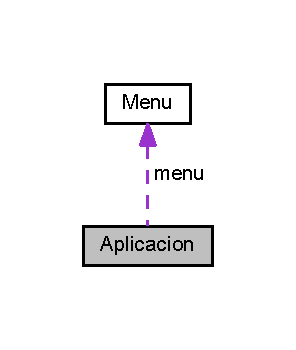
\includegraphics[width=142pt]{class_aplicacion__coll__graph}
\end{center}
\end{figure}
\subsection*{Public Member Functions}
\begin{DoxyCompactItemize}
\item 
{\bf Aplicacion} ()
\item 
{\bf $\sim$\-Aplicacion} ()
\item 
void {\bf iniciar} ()
\item 
void {\bf add\-Pregunta} ({\bf Pregunta} $\ast$input)
\end{DoxyCompactItemize}
\subsection*{Private Member Functions}
\begin{DoxyCompactItemize}
\item 
void {\bf Encuesta} ()
\item 
void {\bf Registros} ()
\end{DoxyCompactItemize}
\subsection*{Private Attributes}
\begin{DoxyCompactItemize}
\item 
bool {\bf final}
\item 
vector$<$ {\bf Pregunta} $\ast$ $>$ {\bf preguntas}
\item 
{\bf Menu} {\bf menu}
\end{DoxyCompactItemize}


\subsection{Detailed Description}


Definition at line 13 of file Aplicacion.\-h.



\subsection{Constructor \& Destructor Documentation}
\index{Aplicacion@{Aplicacion}!Aplicacion@{Aplicacion}}
\index{Aplicacion@{Aplicacion}!Aplicacion@{Aplicacion}}
\subsubsection[{Aplicacion}]{\setlength{\rightskip}{0pt plus 5cm}Aplicacion\-::\-Aplicacion (
\begin{DoxyParamCaption}
{}
\end{DoxyParamCaption}
)}\label{class_aplicacion_a732495f2906cb8b97f035d0b927e6931}


Definition at line 18 of file Aplicacion.\-cpp.


\begin{DoxyCode}
19 \{
20     menu.addOpcion(\textcolor{stringliteral}{"Encuesta"});
21     menu.addOpcion(\textcolor{stringliteral}{"Consulta"});
22     \textcolor{keyword}{final} =\textcolor{keyword}{true};
23 \}
\end{DoxyCode}
\index{Aplicacion@{Aplicacion}!$\sim$\-Aplicacion@{$\sim$\-Aplicacion}}
\index{$\sim$\-Aplicacion@{$\sim$\-Aplicacion}!Aplicacion@{Aplicacion}}
\subsubsection[{$\sim$\-Aplicacion}]{\setlength{\rightskip}{0pt plus 5cm}Aplicacion\-::$\sim$\-Aplicacion (
\begin{DoxyParamCaption}
{}
\end{DoxyParamCaption}
)}\label{class_aplicacion_a664c55738e44ec36338dbc6f38531263}


Definition at line 13 of file Aplicacion.\-cpp.


\begin{DoxyCode}
14 \{
15 
16 \}
\end{DoxyCode}


\subsection{Member Function Documentation}
\index{Aplicacion@{Aplicacion}!add\-Pregunta@{add\-Pregunta}}
\index{add\-Pregunta@{add\-Pregunta}!Aplicacion@{Aplicacion}}
\subsubsection[{add\-Pregunta}]{\setlength{\rightskip}{0pt plus 5cm}void Aplicacion\-::add\-Pregunta (
\begin{DoxyParamCaption}
\item[{{\bf Pregunta} $\ast$}]{input}
\end{DoxyParamCaption}
)}\label{class_aplicacion_aceef1aa7af0799f8a83d6582f7d34783}


Definition at line 58 of file Aplicacion.\-cpp.


\begin{DoxyCode}
59 \{
60     preguntas.push\_back(input);
61 \}
\end{DoxyCode}


Here is the caller graph for this function\-:\nopagebreak
\begin{figure}[H]
\begin{center}
\leavevmode
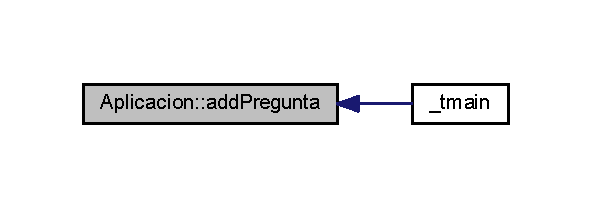
\includegraphics[width=284pt]{class_aplicacion_aceef1aa7af0799f8a83d6582f7d34783_icgraph}
\end{center}
\end{figure}


\index{Aplicacion@{Aplicacion}!Encuesta@{Encuesta}}
\index{Encuesta@{Encuesta}!Aplicacion@{Aplicacion}}
\subsubsection[{Encuesta}]{\setlength{\rightskip}{0pt plus 5cm}void Aplicacion\-::\-Encuesta (
\begin{DoxyParamCaption}
{}
\end{DoxyParamCaption}
)\hspace{0.3cm}{\ttfamily [private]}}\label{class_aplicacion_a593362390998cc4e741cbc0c92319b9e}


Definition at line 44 of file Aplicacion.\-cpp.


\begin{DoxyCode}
45 \{
46     Cuestionario cuestionario(preguntas);\textcolor{comment}{//se crea un cuestionario donde se a�adiran las preguntas y se
       responderan, tambi�n con este objeto se guardaran}
47     \textcolor{comment}{//for (size\_t i=0;i<preguntas.size();i++) \{cuestionario.addPregunta(preguntas[i]);\} //En este ciclo se
       a�aden todas las preguntas del vector al cuestionario}
48 
49     cuestionario.hacerPreguntas();\textcolor{comment}{//con este metodo se imprimien y se contestan las preguntas del
       cuestionario}
50     \textcolor{keywordflow}{if} (cuestionario.GuardarCuestionario()) \textcolor{comment}{//Aqui intenta guardar el cuestionario en un archivo de texto
       "respuestas.txt"}
51     \{
52         cout<<\textcolor{stringliteral}{"Encuesta guardada. Gracias :)"}; \textcolor{comment}{//si se logra guardar, entonces se imprime este mensaje}
53         \textcolor{keyword}{final}=\textcolor{keyword}{false}; \textcolor{comment}{//se asigna esta variable global a 0, para que el hilo principal salga del ciclo y
       entonces pueda cerrarse el programa}
54     \}
55     \textcolor{keywordflow}{else} cout<<\textcolor{stringliteral}{"Error al guardar la encuesta, Contacte al Encargado"}; \textcolor{comment}{//Se imprime este mensaje y no se
       cierra el programa, cuando hay un error al guardar la encuesta}
56 \}
\end{DoxyCode}


Here is the call graph for this function\-:
\nopagebreak
\begin{figure}[H]
\begin{center}
\leavevmode
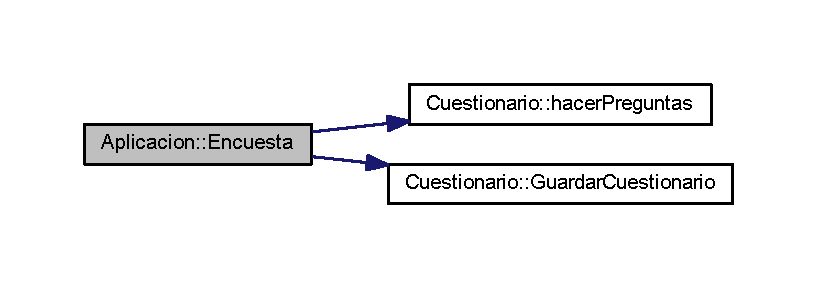
\includegraphics[width=350pt]{class_aplicacion_a593362390998cc4e741cbc0c92319b9e_cgraph}
\end{center}
\end{figure}




Here is the caller graph for this function\-:
\nopagebreak
\begin{figure}[H]
\begin{center}
\leavevmode
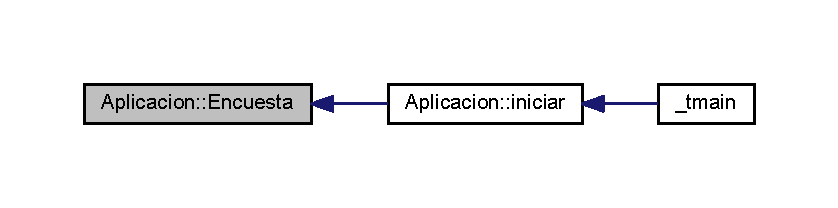
\includegraphics[width=350pt]{class_aplicacion_a593362390998cc4e741cbc0c92319b9e_icgraph}
\end{center}
\end{figure}


\index{Aplicacion@{Aplicacion}!iniciar@{iniciar}}
\index{iniciar@{iniciar}!Aplicacion@{Aplicacion}}
\subsubsection[{iniciar}]{\setlength{\rightskip}{0pt plus 5cm}void Aplicacion\-::iniciar (
\begin{DoxyParamCaption}
{}
\end{DoxyParamCaption}
)}\label{class_aplicacion_a01d38ba3ea36e2201e5e17b9593cc220}


Definition at line 63 of file Aplicacion.\-cpp.


\begin{DoxyCode}
64 \{
65     \textcolor{keywordflow}{if}(!validarAcceso())return ; \textcolor{comment}{//Aqui se checa que la llave este puesta, si no esta se sale del programa,
       s� si est� continua la ejecuci�n encontrada, Favor de elegir la opcion adecuada\(\backslash\)n ";
    thread * hiloElegido = nullptr;
    switch (menu.SeleccionarOpcion())
    \{
    case 1:
        hiloElegido = new thread(&Aplicacion::Encuesta,this);
        break;
    case 2:
        hiloElegido = new thread(&Aplicacion::Registros,this);
        break;
    default:
        final=false;
        break;
    \}


    //thread hiloEjecucion(&Aplicacion::Registros,this); //Aqui se llama as�ncronamente un hilo de
       ejecuci�n, llamando a la funcion previamente definida llamada "AplicacionDeEncuesta"
    this\_thread::sleep\_for(std::chrono::milliseconds(3000)); //Se espera 3 segundos antes de entrar al
       ciclo infinito
    while (validarAcceso()&&final) //Este es el ciclo While que se realiza infinitamente, hasta que la
       encuesta se termine (pues la variable final queda en 0 y dado que 1^0=0) 
    \{
        this\_thread::sleep\_for(std::chrono::milliseconds(3000));//El proceso duerme por 3 segundos antes de
       volver a validar
    \}
    if (hiloElegido!=nullptr)
    \{
        hiloElegido->detach(); //Se destruye el hilo de ejecuci�n de AplicacionDeEncuesta despues de salir del
       ciclo
    \}

    /*string lala[10];
    lala->size();*/
    //cin.getline(new char,1);
\}
}
66     cout<<\textcolor{stringliteral}{"Clave encontrada, Favor de elegir la opcion adecuada\(\backslash\)n "};
67     thread * hiloElegido = \textcolor{keyword}{nullptr};
68     \textcolor{keywordflow}{switch} (menu.SeleccionarOpcion())
69     \{
70     \textcolor{keywordflow}{case} 1:
71         hiloElegido = \textcolor{keyword}{new} thread(&Aplicacion::Encuesta,\textcolor{keyword}{this});
72         \textcolor{keywordflow}{break};
73     \textcolor{keywordflow}{case} 2:
74         hiloElegido = \textcolor{keyword}{new} thread(&Aplicacion::Registros,\textcolor{keyword}{this});
75         \textcolor{keywordflow}{break};
76     \textcolor{keywordflow}{default}:
77         \textcolor{keyword}{final}=\textcolor{keyword}{false};
78         \textcolor{keywordflow}{break};
79     \}
80 
81 
82     \textcolor{comment}{//thread hiloEjecucion(&Aplicacion::Registros,this); //Aqui se llama as�ncronamente un hilo de
       ejecuci�n, llamando a la funcion previamente definida llamada "AplicacionDeEncuesta"}
83     this\_thread::sleep\_for(std::chrono::milliseconds(3000)); \textcolor{comment}{//Se espera 3 segundos antes de entrar al
       ciclo infinito}
84     \textcolor{keywordflow}{while} (validarAcceso()&&\textcolor{keyword}{final}) \textcolor{comment}{//Este es el ciclo While que se realiza infinitamente, hasta que la
       encuesta se termine (pues la variable final queda en 0 y dado que 1^0=0) }
85     \{
86         this\_thread::sleep\_for(std::chrono::milliseconds(3000));\textcolor{comment}{//El proceso duerme por 3 segundos antes de
       volver a validar}
87     \}
88     \textcolor{keywordflow}{if} (hiloElegido!=\textcolor{keyword}{nullptr})
89     \{
90         hiloElegido->detach(); \textcolor{comment}{//Se destruye el hilo de ejecuci�n de AplicacionDeEncuesta despues de salir del
       ciclo}
91     \}
92 
93     \textcolor{comment}{/*string lala[10];}
94 \textcolor{comment}{    lala->size();*/}
95     \textcolor{comment}{//cin.getline(new char,1);}
96 \}
\end{DoxyCode}


Here is the call graph for this function\-:
\nopagebreak
\begin{figure}[H]
\begin{center}
\leavevmode
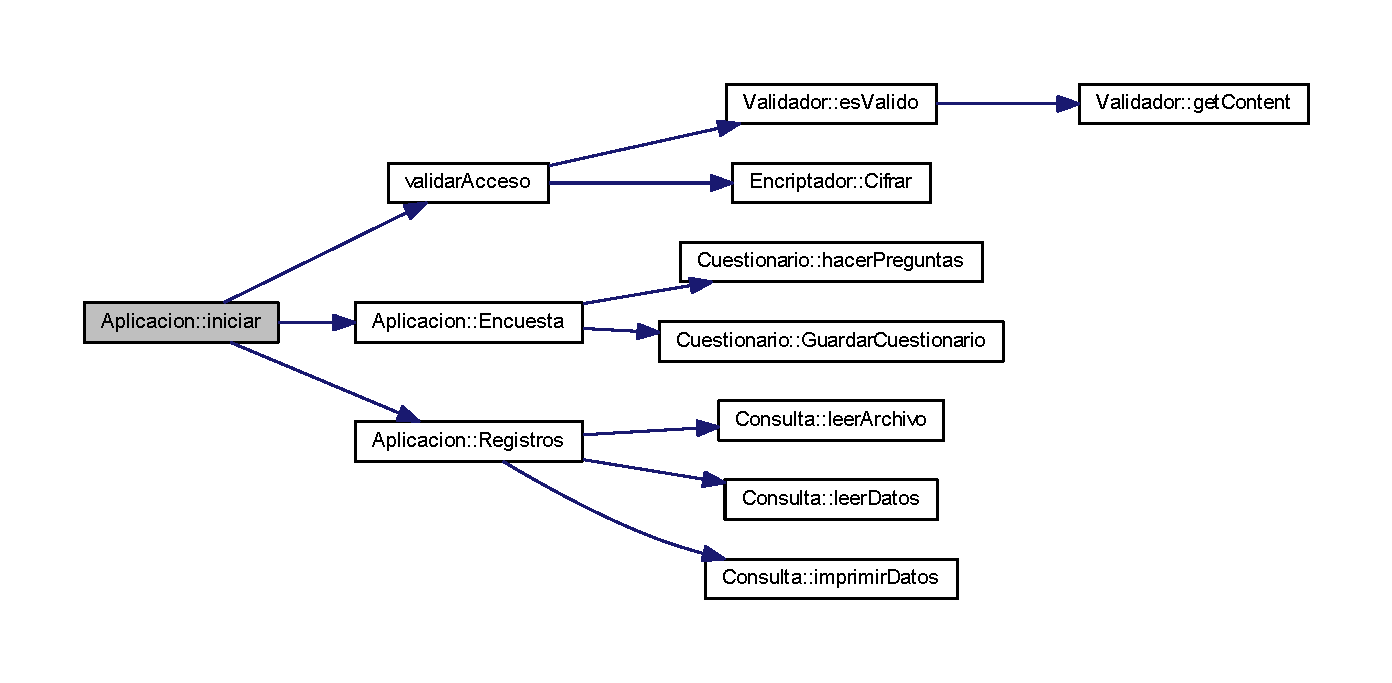
\includegraphics[width=350pt]{class_aplicacion_a01d38ba3ea36e2201e5e17b9593cc220_cgraph}
\end{center}
\end{figure}




Here is the caller graph for this function\-:\nopagebreak
\begin{figure}[H]
\begin{center}
\leavevmode
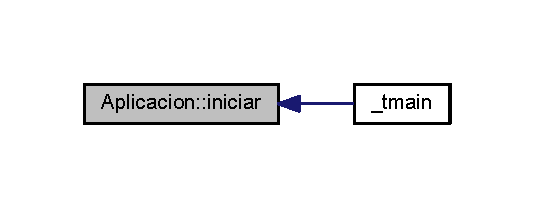
\includegraphics[width=256pt]{class_aplicacion_a01d38ba3ea36e2201e5e17b9593cc220_icgraph}
\end{center}
\end{figure}


\index{Aplicacion@{Aplicacion}!Registros@{Registros}}
\index{Registros@{Registros}!Aplicacion@{Aplicacion}}
\subsubsection[{Registros}]{\setlength{\rightskip}{0pt plus 5cm}void Aplicacion\-::\-Registros (
\begin{DoxyParamCaption}
{}
\end{DoxyParamCaption}
)\hspace{0.3cm}{\ttfamily [private]}}\label{class_aplicacion_abc60d6d5258aa20306798c81d20b91e4}


Definition at line 25 of file Aplicacion.\-cpp.


\begin{DoxyCode}
26 \{
27     Aplicacion();
28     Consulta consulta(preguntas);
29     \textcolor{keywordflow}{if} (consulta.leerArchivo(\textcolor{stringliteral}{"respuesta.txt"}))
30     \{
31         consulta.leerDatos();
32         consulta.imprimirDatos();
33         cin.getline(\textcolor{keyword}{new} \textcolor{keywordtype}{char},1);
34         cin.ignore();
35         \textcolor{keyword}{final}=\textcolor{keyword}{false};
36 
37     \}
38     \textcolor{keywordflow}{else}
39     \{
40         cout<<\textcolor{stringliteral}{"Error al leer el archivo de las respuestas"}<<endl;
41     \}
42 \}
\end{DoxyCode}


Here is the call graph for this function\-:
\nopagebreak
\begin{figure}[H]
\begin{center}
\leavevmode
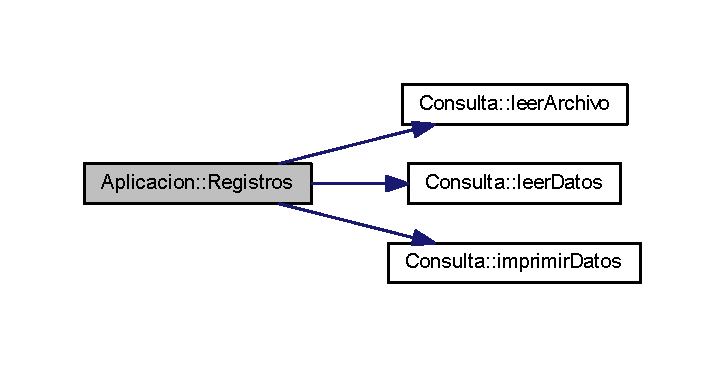
\includegraphics[width=348pt]{class_aplicacion_abc60d6d5258aa20306798c81d20b91e4_cgraph}
\end{center}
\end{figure}




Here is the caller graph for this function\-:
\nopagebreak
\begin{figure}[H]
\begin{center}
\leavevmode
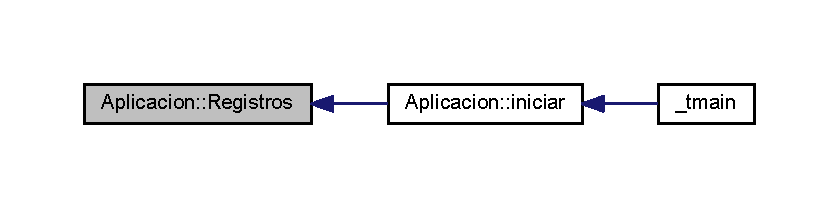
\includegraphics[width=350pt]{class_aplicacion_abc60d6d5258aa20306798c81d20b91e4_icgraph}
\end{center}
\end{figure}




\subsection{Member Data Documentation}
\index{Aplicacion@{Aplicacion}!final@{final}}
\index{final@{final}!Aplicacion@{Aplicacion}}
\subsubsection[{final}]{\setlength{\rightskip}{0pt plus 5cm}bool Aplicacion\-::final\hspace{0.3cm}{\ttfamily [private]}}\label{class_aplicacion_a2469262187eccb4e454a43898ae4586a}


Definition at line 21 of file Aplicacion.\-h.

\index{Aplicacion@{Aplicacion}!menu@{menu}}
\index{menu@{menu}!Aplicacion@{Aplicacion}}
\subsubsection[{menu}]{\setlength{\rightskip}{0pt plus 5cm}{\bf Menu} Aplicacion\-::menu\hspace{0.3cm}{\ttfamily [private]}}\label{class_aplicacion_a22da91ee92f47ee873c2047d9fa14c09}


Definition at line 23 of file Aplicacion.\-h.

\index{Aplicacion@{Aplicacion}!preguntas@{preguntas}}
\index{preguntas@{preguntas}!Aplicacion@{Aplicacion}}
\subsubsection[{preguntas}]{\setlength{\rightskip}{0pt plus 5cm}vector$<${\bf Pregunta}$\ast$$>$ Aplicacion\-::preguntas\hspace{0.3cm}{\ttfamily [private]}}\label{class_aplicacion_aca6c6065e3562fc99904aaaf7254a9bd}


Definition at line 22 of file Aplicacion.\-h.



The documentation for this class was generated from the following files\-:\begin{DoxyCompactItemize}
\item 
Proyecto\-Integrador2/{\bf Aplicacion.\-h}\item 
Proyecto\-Integrador2/{\bf Aplicacion.\-cpp}\end{DoxyCompactItemize}

\section{Consulta Class Reference}
\label{class_consulta}\index{Consulta@{Consulta}}


{\ttfamily \#include $<$Consulta.\-h$>$}

\subsection*{Public Member Functions}
\begin{DoxyCompactItemize}
\item 
{\bf Consulta} ()
\item 
{\bf Consulta} (vector$<$ {\bf Pregunta} $\ast$ $>$ {\bf preguntas})
\item 
{\bf $\sim$\-Consulta} ()
\item 
void {\bf add\-Pregunta} ({\bf Pregunta} $\ast$input)
\item 
bool {\bf leer\-Archivo} (string filename)
\item 
void {\bf leer\-Datos} ()
\item 
void {\bf imprimir\-Datos} ()
\end{DoxyCompactItemize}
\subsection*{Private Attributes}
\begin{DoxyCompactItemize}
\item 
ifstream {\bf archivo}
\item 
vector$<$ vector$<$ string $>$ $>$ {\bf Registros}
\item 
vector$<$ {\bf Pregunta} $\ast$ $>$ {\bf preguntas}
\end{DoxyCompactItemize}


\subsection{Detailed Description}


Definition at line 14 of file Consulta.\-h.



\subsection{Constructor \& Destructor Documentation}
\index{Consulta@{Consulta}!Consulta@{Consulta}}
\index{Consulta@{Consulta}!Consulta@{Consulta}}
\subsubsection[{Consulta}]{\setlength{\rightskip}{0pt plus 5cm}Consulta\-::\-Consulta (
\begin{DoxyParamCaption}
{}
\end{DoxyParamCaption}
)}\label{class_consulta_a941db28c9c5f5606fcbfcbd76a4381a7}


Definition at line 69 of file Consulta.\-cpp.


\begin{DoxyCode}
70 \{
71 
72 \}
\end{DoxyCode}
\index{Consulta@{Consulta}!Consulta@{Consulta}}
\index{Consulta@{Consulta}!Consulta@{Consulta}}
\subsubsection[{Consulta}]{\setlength{\rightskip}{0pt plus 5cm}Consulta\-::\-Consulta (
\begin{DoxyParamCaption}
\item[{vector$<$ {\bf Pregunta} $\ast$ $>$}]{preguntas}
\end{DoxyParamCaption}
)}\label{class_consulta_a57114e4d0b3844a02825595fbc702057}


Definition at line 74 of file Consulta.\-cpp.


\begin{DoxyCode}
75 \{
76     this->preguntas=preguntas;
77 \}
\end{DoxyCode}
\index{Consulta@{Consulta}!$\sim$\-Consulta@{$\sim$\-Consulta}}
\index{$\sim$\-Consulta@{$\sim$\-Consulta}!Consulta@{Consulta}}
\subsubsection[{$\sim$\-Consulta}]{\setlength{\rightskip}{0pt plus 5cm}Consulta\-::$\sim$\-Consulta (
\begin{DoxyParamCaption}
{}
\end{DoxyParamCaption}
)}\label{class_consulta_a619b1ed733470d7553a893227ae5884a}


Definition at line 64 of file Consulta.\-cpp.


\begin{DoxyCode}
65 \{
66 
67 \}
\end{DoxyCode}


\subsection{Member Function Documentation}
\index{Consulta@{Consulta}!add\-Pregunta@{add\-Pregunta}}
\index{add\-Pregunta@{add\-Pregunta}!Consulta@{Consulta}}
\subsubsection[{add\-Pregunta}]{\setlength{\rightskip}{0pt plus 5cm}void Consulta\-::add\-Pregunta (
\begin{DoxyParamCaption}
\item[{{\bf Pregunta} $\ast$}]{input}
\end{DoxyParamCaption}
)}\label{class_consulta_a8654ef3588e92c6907646cd0093ca67f}


Definition at line 9 of file Consulta.\-cpp.


\begin{DoxyCode}
10 \{
11     preguntas.push\_back(input);
12 \}
\end{DoxyCode}
\index{Consulta@{Consulta}!imprimir\-Datos@{imprimir\-Datos}}
\index{imprimir\-Datos@{imprimir\-Datos}!Consulta@{Consulta}}
\subsubsection[{imprimir\-Datos}]{\setlength{\rightskip}{0pt plus 5cm}void Consulta\-::imprimir\-Datos (
\begin{DoxyParamCaption}
{}
\end{DoxyParamCaption}
)}\label{class_consulta_a56df832e41c410cfe15b6fd2a0f82036}


Definition at line 48 of file Consulta.\-cpp.


\begin{DoxyCode}
49 \{
50     \textcolor{keywordflow}{for} (\textcolor{keywordtype}{int} i = 0; i < Registros.size(); i++)
51     \{
52         cout << \textcolor{stringliteral}{"\(\backslash\)nCuestionario #"}<<i+1<<endl;
53         cout<<\textcolor{stringliteral}{"Fecha: "}<<Registros[i][0]<<endl;
54         \textcolor{comment}{//cout<<preguntas.size()<<endl;}
55         \textcolor{keywordflow}{for} (\textcolor{keywordtype}{int} j = 0; j < preguntas.size(); j++)
56         \{
57             preguntas[j]->imprimirPregunta();
58             cout << Registros[i][j+1] << endl;
59         \}
60 
61     \}
62 \}
\end{DoxyCode}


Here is the caller graph for this function\-:
\nopagebreak
\begin{figure}[H]
\begin{center}
\leavevmode
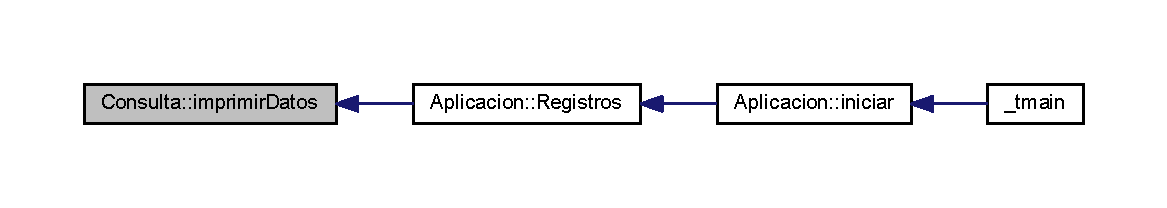
\includegraphics[width=350pt]{class_consulta_a56df832e41c410cfe15b6fd2a0f82036_icgraph}
\end{center}
\end{figure}


\index{Consulta@{Consulta}!leer\-Archivo@{leer\-Archivo}}
\index{leer\-Archivo@{leer\-Archivo}!Consulta@{Consulta}}
\subsubsection[{leer\-Archivo}]{\setlength{\rightskip}{0pt plus 5cm}bool Consulta\-::leer\-Archivo (
\begin{DoxyParamCaption}
\item[{string}]{filename}
\end{DoxyParamCaption}
)}\label{class_consulta_a962f20731f95b0c0e07118da310d8fab}


Definition at line 14 of file Consulta.\-cpp.


\begin{DoxyCode}
15 \{
16     archivo.open(filename,ios::binary|ios::in);
17     \textcolor{comment}{//fs.read(buffer,1000000);}
18     \textcolor{keywordflow}{if}(!archivo)\{
19         \textcolor{keywordflow}{return} \textcolor{keyword}{false};
20     \}
21     \textcolor{keywordflow}{return} \textcolor{keyword}{true};
22 \}
\end{DoxyCode}


Here is the caller graph for this function\-:
\nopagebreak
\begin{figure}[H]
\begin{center}
\leavevmode
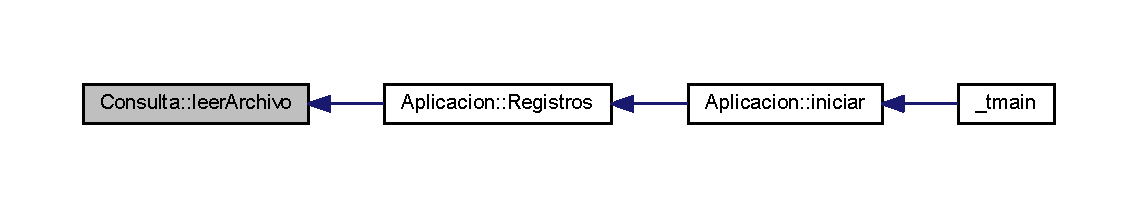
\includegraphics[width=350pt]{class_consulta_a962f20731f95b0c0e07118da310d8fab_icgraph}
\end{center}
\end{figure}


\index{Consulta@{Consulta}!leer\-Datos@{leer\-Datos}}
\index{leer\-Datos@{leer\-Datos}!Consulta@{Consulta}}
\subsubsection[{leer\-Datos}]{\setlength{\rightskip}{0pt plus 5cm}void Consulta\-::leer\-Datos (
\begin{DoxyParamCaption}
{}
\end{DoxyParamCaption}
)}\label{class_consulta_a559e96b607fd1ac665628432f399e0c5}


Definition at line 24 of file Consulta.\-cpp.


\begin{DoxyCode}
25 \{
26     vector<string> Respuestas;
27     \textcolor{keywordtype}{string} temporal=\textcolor{stringliteral}{""};
28     \textcolor{keywordtype}{char} buffer;
29     \textcolor{keywordflow}{while} (archivo.good())
30     \{
31         buffer=archivo.get();
32         \textcolor{keywordflow}{if}(buffer==\textcolor{charliteral}{'\(\backslash\)t'})\{
33             Respuestas.push\_back(temporal);
34             \textcolor{comment}{//cout<<temporal<<endl;}
35             temporal=\textcolor{stringliteral}{""};
36             \textcolor{keywordflow}{continue};
37         \}
38         \textcolor{keywordflow}{if}(buffer==\textcolor{charliteral}{'\(\backslash\)n'})\{
39             Registros.push\_back(Respuestas);
40             Respuestas.clear();
41             \textcolor{comment}{//cout<<"Nuevo Registro"<<endl;}
42             \textcolor{keywordflow}{continue};
43         \}
44         temporal+=buffer;
45     \}
46 \}
\end{DoxyCode}


Here is the caller graph for this function\-:
\nopagebreak
\begin{figure}[H]
\begin{center}
\leavevmode
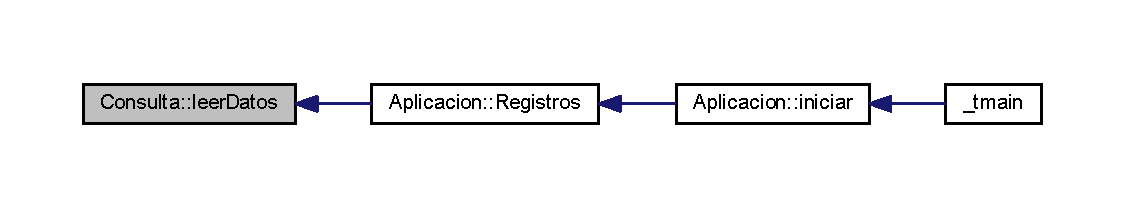
\includegraphics[width=350pt]{class_consulta_a559e96b607fd1ac665628432f399e0c5_icgraph}
\end{center}
\end{figure}




\subsection{Member Data Documentation}
\index{Consulta@{Consulta}!archivo@{archivo}}
\index{archivo@{archivo}!Consulta@{Consulta}}
\subsubsection[{archivo}]{\setlength{\rightskip}{0pt plus 5cm}ifstream Consulta\-::archivo\hspace{0.3cm}{\ttfamily [private]}}\label{class_consulta_aee038d050fa188962105e79e4680f402}


Definition at line 25 of file Consulta.\-h.

\index{Consulta@{Consulta}!preguntas@{preguntas}}
\index{preguntas@{preguntas}!Consulta@{Consulta}}
\subsubsection[{preguntas}]{\setlength{\rightskip}{0pt plus 5cm}vector$<${\bf Pregunta}$\ast$$>$ Consulta\-::preguntas\hspace{0.3cm}{\ttfamily [private]}}\label{class_consulta_a71abff7d94e9294e397319203433bb4d}


Definition at line 27 of file Consulta.\-h.

\index{Consulta@{Consulta}!Registros@{Registros}}
\index{Registros@{Registros}!Consulta@{Consulta}}
\subsubsection[{Registros}]{\setlength{\rightskip}{0pt plus 5cm}vector$<$vector$<$string$>$ $>$ Consulta\-::\-Registros\hspace{0.3cm}{\ttfamily [private]}}\label{class_consulta_a3b014f1cb3635323fea65437c4ba7535}


Definition at line 26 of file Consulta.\-h.



The documentation for this class was generated from the following files\-:\begin{DoxyCompactItemize}
\item 
Proyecto\-Integrador2/{\bf Consulta.\-h}\item 
Proyecto\-Integrador2/{\bf Consulta.\-cpp}\end{DoxyCompactItemize}

\section{Referencia de la Clase Cuestionario}
\label{class_cuestionario}\index{Cuestionario@{Cuestionario}}


{\ttfamily \#include $<$Cuestionario.\-h$>$}

\subsection*{Métodos públicos}
\begin{DoxyCompactItemize}
\item 
{\bf Cuestionario} ()
\item 
{\bf $\sim$\-Cuestionario} ()
\item 
bool {\bf Guardar\-Cuestionario} ()
\item 
void {\bf hacer\-Preguntas} ()
\item 
void {\bf add\-Pregunta} ({\bf Pregunta} $\ast$)
\end{DoxyCompactItemize}


\subsection{Descripción detallada}


Definición en la línea 6 del archivo Cuestionario.\-h.



\subsection{Documentación del constructor y destructor}
\index{Cuestionario@{Cuestionario}!Cuestionario@{Cuestionario}}
\index{Cuestionario@{Cuestionario}!Cuestionario@{Cuestionario}}
\subsubsection[{Cuestionario}]{\setlength{\rightskip}{0pt plus 5cm}Cuestionario\-::\-Cuestionario (
\begin{DoxyParamCaption}
{}
\end{DoxyParamCaption}
)}\label{class_cuestionario_a2455ac26c1e8d11143184e6dbd91e1f4}


Definición en la línea 12 del archivo Cuestionario.\-cpp.


\begin{DoxyCode}
13 \{
14     
15 \}
\end{DoxyCode}
\index{Cuestionario@{Cuestionario}!$\sim$\-Cuestionario@{$\sim$\-Cuestionario}}
\index{$\sim$\-Cuestionario@{$\sim$\-Cuestionario}!Cuestionario@{Cuestionario}}
\subsubsection[{$\sim$\-Cuestionario}]{\setlength{\rightskip}{0pt plus 5cm}Cuestionario\-::$\sim$\-Cuestionario (
\begin{DoxyParamCaption}
{}
\end{DoxyParamCaption}
)}\label{class_cuestionario_af2998a894d70b648fc0a088924cf09f2}


Definición en la línea 17 del archivo Cuestionario.\-cpp.


\begin{DoxyCode}
18 \{
19 
20 \}
\end{DoxyCode}


\subsection{Documentación de las funciones miembro}
\index{Cuestionario@{Cuestionario}!add\-Pregunta@{add\-Pregunta}}
\index{add\-Pregunta@{add\-Pregunta}!Cuestionario@{Cuestionario}}
\subsubsection[{add\-Pregunta}]{\setlength{\rightskip}{0pt plus 5cm}void Cuestionario\-::add\-Pregunta (
\begin{DoxyParamCaption}
\item[{{\bf Pregunta} $\ast$}]{input}
\end{DoxyParamCaption}
)}\label{class_cuestionario_a6fde1365c5b84321eba9a6c03512ae65}


Definición en la línea 64 del archivo Cuestionario.\-cpp.


\begin{DoxyCode}
64                                              \{
65     preguntas.push\_back(input);
66 
67 \}
\end{DoxyCode}


Gráfico de llamadas a esta función\-:
\nopagebreak
\begin{figure}[H]
\begin{center}
\leavevmode
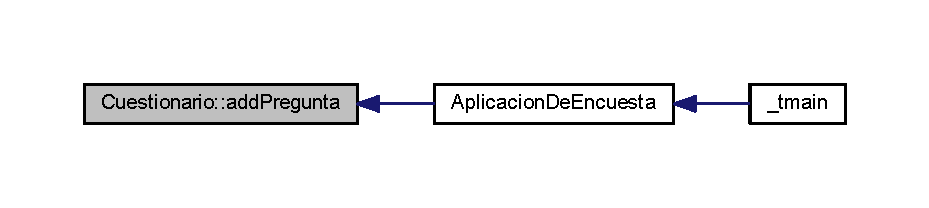
\includegraphics[width=350pt]{class_cuestionario_a6fde1365c5b84321eba9a6c03512ae65_icgraph}
\end{center}
\end{figure}


\index{Cuestionario@{Cuestionario}!Guardar\-Cuestionario@{Guardar\-Cuestionario}}
\index{Guardar\-Cuestionario@{Guardar\-Cuestionario}!Cuestionario@{Cuestionario}}
\subsubsection[{Guardar\-Cuestionario}]{\setlength{\rightskip}{0pt plus 5cm}bool Cuestionario\-::\-Guardar\-Cuestionario (
\begin{DoxyParamCaption}
{}
\end{DoxyParamCaption}
)}\label{class_cuestionario_ab8cf9b63d66a3ab624a2ff0b9f854773}


Definición en la línea 22 del archivo Cuestionario.\-cpp.


\begin{DoxyCode}
23 \{
24     \textcolor{keyword}{typedef} std::chrono::system\_clock Clock;
25     \textcolor{keyword}{auto} now = Clock::now();
26     std::time\_t now\_c = Clock::to\_time\_t(now);
27 
28     \textcolor{keyword}{struct }tm *parts = std::localtime(&now\_c);
29     \textcolor{keywordtype}{int} anio= 1900 + parts->tm\_year;
30     \textcolor{keywordtype}{int} month= 1    + parts->tm\_mon;
31     \textcolor{keywordtype}{int} day = parts->tm\_mday ;
32 
33     ofstream myfile;
34     myfile.open(\textcolor{stringliteral}{"respuesta.txt"},ios::out | ios::app);
35     \textcolor{keywordtype}{string} respues = \textcolor{stringliteral}{""};
36     \textcolor{keywordflow}{if} (myfile.is\_open())
37     \{
38         \textcolor{keywordflow}{for} (\textcolor{keywordtype}{size\_t} i=0;i<preguntas.size();i++)
39         \{
40             respues+=preguntas[i]->getRespuesta()+\textcolor{stringliteral}{"\(\backslash\)t"};
41         \}
42         myfile << 1900 + parts->tm\_year  << \textcolor{stringliteral}{"\_"};
43         myfile << 1    + parts->tm\_mon   << \textcolor{stringliteral}{"\_"};
44         myfile <<        parts->tm\_mday  << \textcolor{stringliteral}{"\(\backslash\)t"};
45         myfile << respues <<\textcolor{stringliteral}{"\(\backslash\)n"};
46         myfile.close();
47         \textcolor{keywordflow}{return} \textcolor{keyword}{true};
48     \}
49     \textcolor{keywordflow}{else} cout << \textcolor{stringliteral}{"No se puede guardar"};
50     \textcolor{keywordflow}{return} \textcolor{keyword}{false};
51 \}
\end{DoxyCode}


Gráfico de llamadas a esta función\-:
\nopagebreak
\begin{figure}[H]
\begin{center}
\leavevmode
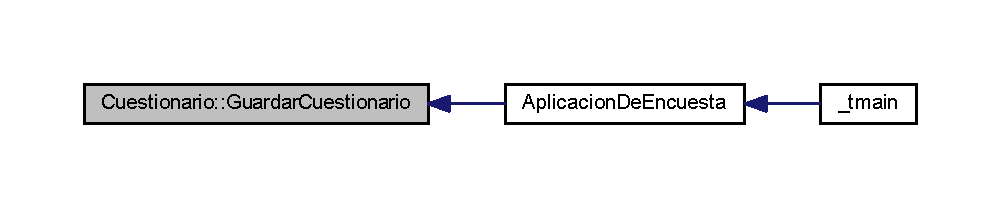
\includegraphics[width=350pt]{class_cuestionario_ab8cf9b63d66a3ab624a2ff0b9f854773_icgraph}
\end{center}
\end{figure}


\index{Cuestionario@{Cuestionario}!hacer\-Preguntas@{hacer\-Preguntas}}
\index{hacer\-Preguntas@{hacer\-Preguntas}!Cuestionario@{Cuestionario}}
\subsubsection[{hacer\-Preguntas}]{\setlength{\rightskip}{0pt plus 5cm}void Cuestionario\-::hacer\-Preguntas (
\begin{DoxyParamCaption}
{}
\end{DoxyParamCaption}
)}\label{class_cuestionario_ae79115ce61bd16dbd5850756035aa2b2}


Definición en la línea 53 del archivo Cuestionario.\-cpp.


\begin{DoxyCode}
54 \{
55     \textcolor{keywordtype}{int} numeroPreguntas = this->preguntas.size();
56 \textcolor{comment}{//  cout<<preguntas.size()<<"eltama~no\(\backslash\)n";}
57     \textcolor{keywordflow}{for} (\textcolor{keywordtype}{int} contadorPreguntas=0;contadorPreguntas<numeroPreguntas;contadorPreguntas++)
58     \{
59         preguntas[contadorPreguntas]->imprimirPregunta();
60         preguntas[contadorPreguntas]->responder();
61     \}
62 \}
\end{DoxyCode}


Gráfico de llamadas a esta función\-:
\nopagebreak
\begin{figure}[H]
\begin{center}
\leavevmode
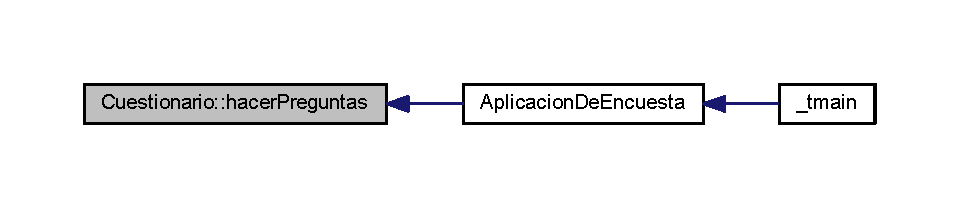
\includegraphics[width=350pt]{class_cuestionario_ae79115ce61bd16dbd5850756035aa2b2_icgraph}
\end{center}
\end{figure}




La documentación para esta clase fue generada a partir de los siguientes ficheros\-:\begin{DoxyCompactItemize}
\item 
Proyecto\-Integrador2/{\bf Cuestionario.\-h}\item 
Proyecto\-Integrador2/{\bf Cuestionario.\-cpp}\end{DoxyCompactItemize}

\section{Encriptador Class Reference}
\label{class_encriptador}\index{Encriptador@{Encriptador}}


{\ttfamily \#include $<$Encriptador.\-h$>$}

\subsection*{Public Member Functions}
\begin{DoxyCompactItemize}
\item 
{\bf Encriptador} (std\-::string clave\-E, std\-::string clave\-D)
\item 
{\bf $\sim$\-Encriptador} ()
\item 
std\-::string {\bf Cifrar} (std\-::string input)
\item 
std\-::string {\bf Decifrar} (std\-::string input)
\end{DoxyCompactItemize}
\subsection*{Private Attributes}
\begin{DoxyCompactItemize}
\item 
std\-::string {\bf clave\-Encriptacion}
\item 
std\-::string {\bf clave\-Desencriptacion}
\item 
int {\bf tamano\-Clave}
\end{DoxyCompactItemize}


\subsection{Detailed Description}


Definition at line 16 of file Encriptador.\-h.



\subsection{Constructor \& Destructor Documentation}
\index{Encriptador@{Encriptador}!Encriptador@{Encriptador}}
\index{Encriptador@{Encriptador}!Encriptador@{Encriptador}}
\subsubsection[{Encriptador}]{\setlength{\rightskip}{0pt plus 5cm}Encriptador\-::\-Encriptador (
\begin{DoxyParamCaption}
\item[{std\-::string}]{clave\-E, }
\item[{std\-::string}]{clave\-D}
\end{DoxyParamCaption}
)}\label{class_encriptador_a35b3d94b703958c627475852edd349bc}


Definition at line 51 of file Encriptador.\-cpp.


\begin{DoxyCode}
52 \{
53     \textcolor{keywordflow}{if} (claveE.length() != claveD.length())
54     \{
55         \textcolor{keywordflow}{return};
56     \}
57     claveEncriptacion=claveE;
58     claveDesencriptacion=claveD;
59     tamanoClave = claveD.length()-1;
60 \}
\end{DoxyCode}
\index{Encriptador@{Encriptador}!$\sim$\-Encriptador@{$\sim$\-Encriptador}}
\index{$\sim$\-Encriptador@{$\sim$\-Encriptador}!Encriptador@{Encriptador}}
\subsubsection[{$\sim$\-Encriptador}]{\setlength{\rightskip}{0pt plus 5cm}Encriptador\-::$\sim$\-Encriptador (
\begin{DoxyParamCaption}
{}
\end{DoxyParamCaption}
)}\label{class_encriptador_a93024926b47a3da38bd8b3ff83c5fb84}


Definition at line 46 of file Encriptador.\-cpp.


\begin{DoxyCode}
47 \{
48 
49 \}
\end{DoxyCode}


\subsection{Member Function Documentation}
\index{Encriptador@{Encriptador}!Cifrar@{Cifrar}}
\index{Cifrar@{Cifrar}!Encriptador@{Encriptador}}
\subsubsection[{Cifrar}]{\setlength{\rightskip}{0pt plus 5cm}std\-::string Encriptador\-::\-Cifrar (
\begin{DoxyParamCaption}
\item[{std\-::string}]{input}
\end{DoxyParamCaption}
)}\label{class_encriptador_aec4f517051f7255e45a6db0f90e21bd4}


Definition at line 29 of file Encriptador.\-cpp.


\begin{DoxyCode}
30 \{
31     \textcolor{keywordflow}{for} (\textcolor{keywordtype}{size\_t} i =0;i<input.length();i++)
32     \{
33         \textcolor{keywordtype}{int} posE = claveDesencriptacion.find(input[i]);
34         \textcolor{keywordtype}{int} posF = posE+i;
35         \textcolor{keywordflow}{if} (posF>tamanoClave) posF = ((posE+i)%tamanoClave)-1;
36         \textcolor{keywordflow}{if}(posE != std::string::npos)input[i]=claveEncriptacion[posF];
37         \textcolor{keywordflow}{else} input[i]=\textcolor{charliteral}{'#'};
38         \textcolor{comment}{//std::cout<<posF<<"<Pf Tc>"<<tamanoClave<<std::endl;}
39     \}
40 
41 
42 
43     \textcolor{keywordflow}{return} input;
44 \}
\end{DoxyCode}


Here is the caller graph for this function\-:\nopagebreak
\begin{figure}[H]
\begin{center}
\leavevmode
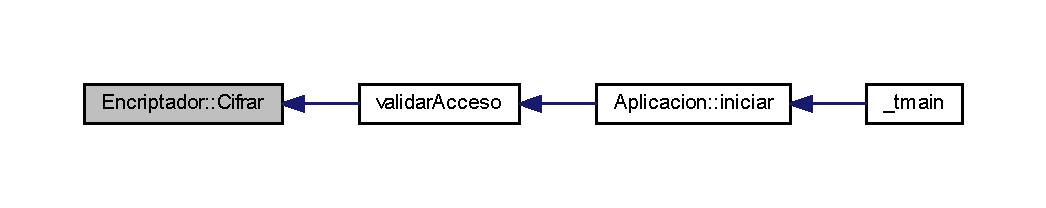
\includegraphics[width=350pt]{class_encriptador_aec4f517051f7255e45a6db0f90e21bd4_icgraph}
\end{center}
\end{figure}


\index{Encriptador@{Encriptador}!Decifrar@{Decifrar}}
\index{Decifrar@{Decifrar}!Encriptador@{Encriptador}}
\subsubsection[{Decifrar}]{\setlength{\rightskip}{0pt plus 5cm}std\-::string Encriptador\-::\-Decifrar (
\begin{DoxyParamCaption}
\item[{std\-::string}]{input}
\end{DoxyParamCaption}
)}\label{class_encriptador_a7e00b65cf581293b47f126506f8c5b42}


Definition at line 10 of file Encriptador.\-cpp.


\begin{DoxyCode}
11 \{
12     \textcolor{keywordflow}{for} (\textcolor{keywordtype}{size\_t} i =0;i<input.length();i++)
13     \{
14         \textcolor{keywordtype}{int} posE = claveEncriptacion.find(input[i]);
15         \textcolor{keywordtype}{int} posF = posE - i;
16         \textcolor{keywordflow}{if} (posF<0)
17         \{
18             posF %= tamanoClave;
19             posF += tamanoClave;
20             posF++;
21         \}
22         \textcolor{keywordflow}{if}(posE != std::string::npos)input[i]=claveDesencriptacion[posF];
23         \textcolor{keywordflow}{else} input[i]=\textcolor{charliteral}{'#'};
24         \textcolor{comment}{//std::cout<<posF<<"<Pf Tc>"<<tamanoClave<<std::endl;}
25     \}
26     \textcolor{keywordflow}{return} input;
27 \}
\end{DoxyCode}


\subsection{Member Data Documentation}
\index{Encriptador@{Encriptador}!clave\-Desencriptacion@{clave\-Desencriptacion}}
\index{clave\-Desencriptacion@{clave\-Desencriptacion}!Encriptador@{Encriptador}}
\subsubsection[{clave\-Desencriptacion}]{\setlength{\rightskip}{0pt plus 5cm}std\-::string Encriptador\-::clave\-Desencriptacion\hspace{0.3cm}{\ttfamily [private]}}\label{class_encriptador_a70a589e464dee2e417bb14a87cf458ca}


Definition at line 25 of file Encriptador.\-h.

\index{Encriptador@{Encriptador}!clave\-Encriptacion@{clave\-Encriptacion}}
\index{clave\-Encriptacion@{clave\-Encriptacion}!Encriptador@{Encriptador}}
\subsubsection[{clave\-Encriptacion}]{\setlength{\rightskip}{0pt plus 5cm}std\-::string Encriptador\-::clave\-Encriptacion\hspace{0.3cm}{\ttfamily [private]}}\label{class_encriptador_a2556c08307108e435116ae4cffbd9ef8}


Definition at line 24 of file Encriptador.\-h.

\index{Encriptador@{Encriptador}!tamano\-Clave@{tamano\-Clave}}
\index{tamano\-Clave@{tamano\-Clave}!Encriptador@{Encriptador}}
\subsubsection[{tamano\-Clave}]{\setlength{\rightskip}{0pt plus 5cm}int Encriptador\-::tamano\-Clave\hspace{0.3cm}{\ttfamily [private]}}\label{class_encriptador_a4fb1a20c261b9a3aa7a975af581969a5}


Definition at line 26 of file Encriptador.\-h.



The documentation for this class was generated from the following files\-:\begin{DoxyCompactItemize}
\item 
Proyecto\-Integrador2/{\bf Encriptador.\-h}\item 
Proyecto\-Integrador2/{\bf Encriptador.\-cpp}\end{DoxyCompactItemize}

\section{Menu Class Reference}
\label{class_menu}\index{Menu@{Menu}}


{\ttfamily \#include $<$Menu.\-h$>$}

\subsection*{Public Member Functions}
\begin{DoxyCompactItemize}
\item 
{\bf Menu} ()
\item 
{\bf Menu} (vector$<$ string $>$ {\bf opciones})
\item 
int {\bf Seleccionar\-Opcion} ()
\item 
void {\bf add\-Opcion} (string opcion)
\end{DoxyCompactItemize}
\subsection*{Private Attributes}
\begin{DoxyCompactItemize}
\item 
vector$<$ string $>$ {\bf opciones}
\item 
int {\bf opc}
\end{DoxyCompactItemize}


\subsection{Detailed Description}


Definition at line 10 of file Menu.\-h.



\subsection{Constructor \& Destructor Documentation}
\index{Menu@{Menu}!Menu@{Menu}}
\index{Menu@{Menu}!Menu@{Menu}}
\subsubsection[{Menu}]{\setlength{\rightskip}{0pt plus 5cm}Menu\-::\-Menu (
\begin{DoxyParamCaption}
{}
\end{DoxyParamCaption}
)}\label{class_menu_ad466dd83355124a6ed958430450bfe94}


Definition at line 9 of file Menu.\-cpp.


\begin{DoxyCode}
10 \{
11     opc=0;
12 \}
\end{DoxyCode}
\index{Menu@{Menu}!Menu@{Menu}}
\index{Menu@{Menu}!Menu@{Menu}}
\subsubsection[{Menu}]{\setlength{\rightskip}{0pt plus 5cm}Menu\-::\-Menu (
\begin{DoxyParamCaption}
\item[{vector$<$ string $>$}]{opciones}
\end{DoxyParamCaption}
)}\label{class_menu_a9f671c44dddc15c1fe6684a78ee9a0b9}


Definition at line 14 of file Menu.\-cpp.


\begin{DoxyCode}
15 \{
16     Menu();
17     this->opciones=opciones;
18 \}
\end{DoxyCode}


\subsection{Member Function Documentation}
\index{Menu@{Menu}!add\-Opcion@{add\-Opcion}}
\index{add\-Opcion@{add\-Opcion}!Menu@{Menu}}
\subsubsection[{add\-Opcion}]{\setlength{\rightskip}{0pt plus 5cm}void Menu\-::add\-Opcion (
\begin{DoxyParamCaption}
\item[{string}]{opcion}
\end{DoxyParamCaption}
)}\label{class_menu_ae08a622a2d8ff638bba3f519f3e8365b}


Definition at line 55 of file Menu.\-cpp.


\begin{DoxyCode}
56 \{
57     opciones.push\_back(opcion);
58 \}
\end{DoxyCode}
\index{Menu@{Menu}!Seleccionar\-Opcion@{Seleccionar\-Opcion}}
\index{Seleccionar\-Opcion@{Seleccionar\-Opcion}!Menu@{Menu}}
\subsubsection[{Seleccionar\-Opcion}]{\setlength{\rightskip}{0pt plus 5cm}int Menu\-::\-Seleccionar\-Opcion (
\begin{DoxyParamCaption}
{}
\end{DoxyParamCaption}
)}\label{class_menu_a26b1166a834792bd13e4d0aa06314471}


Definition at line 20 of file Menu.\-cpp.


\begin{DoxyCode}
21 \{
22     \textcolor{comment}{//int opc=0; //opcion del Menu}
23     \textcolor{keywordflow}{while} (opc!=(opciones.size()+1))\textcolor{comment}{//Imprimir el Menu hasta que se seleccione salir(opcion 3)}
24     \{
25         \textcolor{keywordflow}{do}\{
26             system(\textcolor{stringliteral}{"cls"});
27             \textcolor{comment}{//cout << "------------------------ Menu -------------------------" << endl ;}
28             cout << \textcolor{stringliteral}{"-------Elija la opcion que desea realizar---------: "} << endl << endl ;
29             \textcolor{keywordflow}{for} (\textcolor{keywordtype}{size\_t} i = 0; i < opciones.size(); i++)
30             \{
31                 cout<<(i+1)<<\textcolor{stringliteral}{".- "}<<opciones[i]<<\textcolor{stringliteral}{"."}<<endl;
32             \}
33             cout << (opciones.size()+1) <<\textcolor{stringliteral}{".- Salir."} << endl ;
34             cout << \textcolor{stringliteral}{"Seleccionado: "};
35             \textcolor{comment}{//cin.ignore();}
36             opc = \_getche()-48;
37             \textcolor{keywordflow}{if}( opc<1 || opc >(\textcolor{keywordtype}{int})(opciones.size()+1))
38             \{
39                 cout << \textcolor{stringliteral}{"Ese numero no es una opcion, vuelve a ingresar tu opcion."} <<endl;
40                 opc=0;
41 
42                 \textcolor{comment}{//system("pause");}
43             \}
44             \textcolor{keywordflow}{else}
45             \{
46                 \textcolor{comment}{//6cin.ignore();}
47                 \textcolor{keywordflow}{return} opc;
48             \}
49         \}\textcolor{keywordflow}{while}(\textcolor{keyword}{true}); \textcolor{comment}{//condicional}
50         \textcolor{comment}{//cout << "Switch para las opciones";}
51     \}
52     \textcolor{keywordflow}{return} -1;
53 \}
\end{DoxyCode}


\subsection{Member Data Documentation}
\index{Menu@{Menu}!opc@{opc}}
\index{opc@{opc}!Menu@{Menu}}
\subsubsection[{opc}]{\setlength{\rightskip}{0pt plus 5cm}int Menu\-::opc\hspace{0.3cm}{\ttfamily [private]}}\label{class_menu_adc288494315cce3604f06e521d13b0e4}


Definition at line 22 of file Menu.\-h.

\index{Menu@{Menu}!opciones@{opciones}}
\index{opciones@{opciones}!Menu@{Menu}}
\subsubsection[{opciones}]{\setlength{\rightskip}{0pt plus 5cm}vector$<$string$>$ Menu\-::opciones\hspace{0.3cm}{\ttfamily [private]}}\label{class_menu_ab0be6758428c7115eca65679112f1d65}


Definition at line 21 of file Menu.\-h.



The documentation for this class was generated from the following files\-:\begin{DoxyCompactItemize}
\item 
Proyecto\-Integrador2/{\bf Menu.\-h}\item 
Proyecto\-Integrador2/{\bf Menu.\-cpp}\end{DoxyCompactItemize}

\section{Referencia de la Clase Pregunta}
\label{class_pregunta}\index{Pregunta@{Pregunta}}


{\ttfamily \#include $<$Preguntas.\-h$>$}



Diagrama de herencias de Pregunta
\nopagebreak
\begin{figure}[H]
\begin{center}
\leavevmode
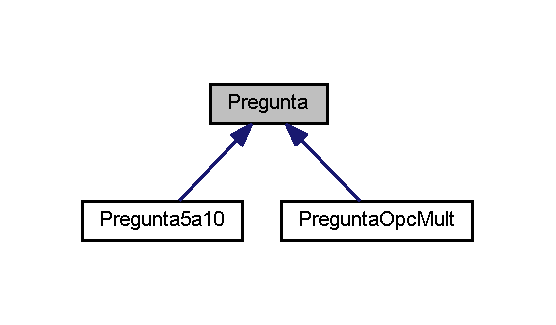
\includegraphics[width=267pt]{class_pregunta__inherit__graph}
\end{center}
\end{figure}
\subsection*{Métodos públicos}
\begin{DoxyCompactItemize}
\item 
{\bf Pregunta} (std\-::string)
\item 
{\bf $\sim$\-Pregunta} ()
\item 
virtual void {\bf responder} ()
\item 
virtual void {\bf imprimir\-Pregunta} ()
\item 
std\-::string {\bf get\-Respuesta} ()
\end{DoxyCompactItemize}
\subsection*{Atributos protegidos}
\begin{DoxyCompactItemize}
\item 
char {\bf respuesta} [512]
\end{DoxyCompactItemize}


\subsection{Descripción detallada}


Definición en la línea 6 del archivo Preguntas.\-h.



\subsection{Documentación del constructor y destructor}
\index{Pregunta@{Pregunta}!Pregunta@{Pregunta}}
\index{Pregunta@{Pregunta}!Pregunta@{Pregunta}}
\subsubsection[{Pregunta}]{\setlength{\rightskip}{0pt plus 5cm}Pregunta\-::\-Pregunta (
\begin{DoxyParamCaption}
\item[{std\-::string}]{pregunta}
\end{DoxyParamCaption}
)}\label{class_pregunta_a24d53ffa52bdb9082366a415dec538d4}


Definición en la línea 9 del archivo Preguntas.\-cpp.


\begin{DoxyCode}
10 \{
11     this->pregunta=pregunta;
12     \textcolor{keywordflow}{for} (\textcolor{keywordtype}{int} i = 0; i < 512; i++)
13     \{
14         respuesta[i]=\textcolor{charliteral}{'\(\backslash\)0'};
15     \}
16 \}
\end{DoxyCode}
\index{Pregunta@{Pregunta}!$\sim$\-Pregunta@{$\sim$\-Pregunta}}
\index{$\sim$\-Pregunta@{$\sim$\-Pregunta}!Pregunta@{Pregunta}}
\subsubsection[{$\sim$\-Pregunta}]{\setlength{\rightskip}{0pt plus 5cm}Pregunta\-::$\sim$\-Pregunta (
\begin{DoxyParamCaption}
{}
\end{DoxyParamCaption}
)\hspace{0.3cm}{\ttfamily [inline]}}\label{class_pregunta_a644894e8c4158aebd9e4ce443c59a0e4}


Definición en la línea 10 del archivo Preguntas.\-h.


\begin{DoxyCode}
10 \{\};
\end{DoxyCode}


\subsection{Documentación de las funciones miembro}
\index{Pregunta@{Pregunta}!get\-Respuesta@{get\-Respuesta}}
\index{get\-Respuesta@{get\-Respuesta}!Pregunta@{Pregunta}}
\subsubsection[{get\-Respuesta}]{\setlength{\rightskip}{0pt plus 5cm}std\-::string Pregunta\-::get\-Respuesta (
\begin{DoxyParamCaption}
{}
\end{DoxyParamCaption}
)}\label{class_pregunta_af7a75dd736d793e35133b0c50fbedb5f}


Definición en la línea 41 del archivo Preguntas.\-cpp.


\begin{DoxyCode}
42 \{
43     \textcolor{keywordflow}{return} *(\textcolor{keyword}{new} string(respuesta));
44 \}
\end{DoxyCode}
\index{Pregunta@{Pregunta}!imprimir\-Pregunta@{imprimir\-Pregunta}}
\index{imprimir\-Pregunta@{imprimir\-Pregunta}!Pregunta@{Pregunta}}
\subsubsection[{imprimir\-Pregunta}]{\setlength{\rightskip}{0pt plus 5cm}void Pregunta\-::imprimir\-Pregunta (
\begin{DoxyParamCaption}
{}
\end{DoxyParamCaption}
)\hspace{0.3cm}{\ttfamily [virtual]}}\label{class_pregunta_ac97860f3cd3d11c415e8cde6e529d7b9}


Reimplementado en {\bf Pregunta\-Opc\-Mult} \doxyref{}{p.}{class_pregunta_opc_mult_a2c87b73c52b7f65956f4a3bcb55ac719} y {\bf Pregunta5a10} \doxyref{}{p.}{class_pregunta5a10_a07d0d7ba39af31469fdfc0a7f4c39e7d}.



Definición en la línea 36 del archivo Preguntas.\-cpp.


\begin{DoxyCode}
37 \{
38     cout<<\textcolor{stringliteral}{"\(\backslash\)n>> "}<<pregunta<<\textcolor{stringliteral}{": "};
39 \}
\end{DoxyCode}
\index{Pregunta@{Pregunta}!responder@{responder}}
\index{responder@{responder}!Pregunta@{Pregunta}}
\subsubsection[{responder}]{\setlength{\rightskip}{0pt plus 5cm}void Pregunta\-::responder (
\begin{DoxyParamCaption}
{}
\end{DoxyParamCaption}
)\hspace{0.3cm}{\ttfamily [virtual]}}\label{class_pregunta_aaf28e3a833e98b6b8bbd9267311a1ad2}


Reimplementado en {\bf Pregunta\-Opc\-Mult} \doxyref{}{p.}{class_pregunta_opc_mult_aaae8febba0ce55b1b2682c8093f6b594} y {\bf Pregunta5a10} \doxyref{}{p.}{class_pregunta5a10_aae1286ae330a08f99bc2edf4bc6b1dd3}.



Definición en la línea 18 del archivo Preguntas.\-cpp.


\begin{DoxyCode}
19 \{
20     \textcolor{comment}{//cin.ignore();}
21 \textcolor{comment}{//  this->imprimirPregunta();}
22     cin.getline(respuesta,512);
23     \textcolor{keywordflow}{for} (\textcolor{keywordtype}{int} i=0;i<512;i++)
24     \{
25         \textcolor{keywordflow}{if} (respuesta[i]==\textcolor{charliteral}{'\(\backslash\)0'})
26         \{
27             \textcolor{keywordflow}{break};
28         \}
29         \textcolor{keywordflow}{if} (respuesta[i]==\textcolor{charliteral}{'\(\backslash\)t'})
30         \{
31             respuesta[i]=\textcolor{charliteral}{' '};
32         \}
33     \}
34 \}
\end{DoxyCode}


\subsection{Documentación de los datos miembro}
\index{Pregunta@{Pregunta}!respuesta@{respuesta}}
\index{respuesta@{respuesta}!Pregunta@{Pregunta}}
\subsubsection[{respuesta}]{\setlength{\rightskip}{0pt plus 5cm}char Pregunta\-::respuesta[512]\hspace{0.3cm}{\ttfamily [protected]}}\label{class_pregunta_a4143cf5905f04f96c035ad12dd5dc9d2}


Definición en la línea 17 del archivo Preguntas.\-h.



La documentación para esta clase fue generada a partir de los siguientes ficheros\-:\begin{DoxyCompactItemize}
\item 
Proyecto\-Integrador2/{\bf Preguntas.\-h}\item 
Proyecto\-Integrador2/{\bf Preguntas.\-cpp}\end{DoxyCompactItemize}

\section{Referencia de la Clase Pregunta5a10}
\label{class_pregunta5a10}\index{Pregunta5a10@{Pregunta5a10}}


{\ttfamily \#include $<$Preguntas.\-h$>$}



Diagrama de herencias de Pregunta5a10
\nopagebreak
\begin{figure}[H]
\begin{center}
\leavevmode
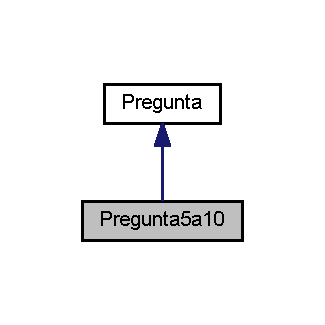
\includegraphics[width=156pt]{class_pregunta5a10__inherit__graph}
\end{center}
\end{figure}


Diagrama de colaboración para Pregunta5a10\-:
\nopagebreak
\begin{figure}[H]
\begin{center}
\leavevmode
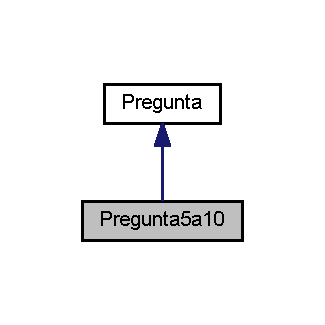
\includegraphics[width=156pt]{class_pregunta5a10__coll__graph}
\end{center}
\end{figure}
\subsection*{Métodos públicos}
\begin{DoxyCompactItemize}
\item 
{\bf Pregunta5a10} (std\-::string)
\item 
{\bf $\sim$\-Pregunta5a10} ()
\item 
void {\bf responder} ()
\item 
void {\bf imprimir\-Pregunta} ()
\end{DoxyCompactItemize}
\subsection*{Otros miembros heredados}


\subsection{Descripción detallada}


Definición en la línea 20 del archivo Preguntas.\-h.



\subsection{Documentación del constructor y destructor}
\index{Pregunta5a10@{Pregunta5a10}!Pregunta5a10@{Pregunta5a10}}
\index{Pregunta5a10@{Pregunta5a10}!Pregunta5a10@{Pregunta5a10}}
\subsubsection[{Pregunta5a10}]{\setlength{\rightskip}{0pt plus 5cm}Pregunta5a10\-::\-Pregunta5a10 (
\begin{DoxyParamCaption}
\item[{std\-::string}]{input}
\end{DoxyParamCaption}
)}\label{class_pregunta5a10_a14ee3b706f038cdfd776c181f319c5eb}


Definición en la línea 46 del archivo Preguntas.\-cpp.


\begin{DoxyCode}
46                                            : Pregunta(input)
47 \{
48 
49 \}
\end{DoxyCode}
\index{Pregunta5a10@{Pregunta5a10}!$\sim$\-Pregunta5a10@{$\sim$\-Pregunta5a10}}
\index{$\sim$\-Pregunta5a10@{$\sim$\-Pregunta5a10}!Pregunta5a10@{Pregunta5a10}}
\subsubsection[{$\sim$\-Pregunta5a10}]{\setlength{\rightskip}{0pt plus 5cm}Pregunta5a10\-::$\sim$\-Pregunta5a10 (
\begin{DoxyParamCaption}
{}
\end{DoxyParamCaption}
)\hspace{0.3cm}{\ttfamily [inline]}}\label{class_pregunta5a10_a41e8af073770d49abb8706f1850822d8}


Definición en la línea 24 del archivo Preguntas.\-h.


\begin{DoxyCode}
24 \{\};
\end{DoxyCode}


\subsection{Documentación de las funciones miembro}
\index{Pregunta5a10@{Pregunta5a10}!imprimir\-Pregunta@{imprimir\-Pregunta}}
\index{imprimir\-Pregunta@{imprimir\-Pregunta}!Pregunta5a10@{Pregunta5a10}}
\subsubsection[{imprimir\-Pregunta}]{\setlength{\rightskip}{0pt plus 5cm}void Pregunta5a10\-::imprimir\-Pregunta (
\begin{DoxyParamCaption}
{}
\end{DoxyParamCaption}
)\hspace{0.3cm}{\ttfamily [virtual]}}\label{class_pregunta5a10_a07d0d7ba39af31469fdfc0a7f4c39e7d}


Reimplementado de {\bf Pregunta} \doxyref{}{p.}{class_pregunta_ac97860f3cd3d11c415e8cde6e529d7b9}.



Definición en la línea 66 del archivo Preguntas.\-cpp.


\begin{DoxyCode}
67 \{
68     \textcolor{comment}{//Pregunta::imprimirPregunta();}
69     \_\_super::imprimirPregunta();
70     cout<<\textcolor{stringliteral}{" (5 a 10) | "};
71 \}
\end{DoxyCode}
\index{Pregunta5a10@{Pregunta5a10}!responder@{responder}}
\index{responder@{responder}!Pregunta5a10@{Pregunta5a10}}
\subsubsection[{responder}]{\setlength{\rightskip}{0pt plus 5cm}void Pregunta5a10\-::responder (
\begin{DoxyParamCaption}
{}
\end{DoxyParamCaption}
)\hspace{0.3cm}{\ttfamily [virtual]}}\label{class_pregunta5a10_aae1286ae330a08f99bc2edf4bc6b1dd3}


Reimplementado de {\bf Pregunta} \doxyref{}{p.}{class_pregunta_aaf28e3a833e98b6b8bbd9267311a1ad2}.



Definición en la línea 51 del archivo Preguntas.\-cpp.


\begin{DoxyCode}
52 \{
53 \textcolor{comment}{//  imprimirPregunta();}
54 \_\_super::responder();
55 \textcolor{comment}{//cout<<respuesta<<"res\(\backslash\)n";}
56 istringstream ss(respuesta);
57 \textcolor{keywordtype}{int} x;
58 \textcolor{keywordflow}{if} (!(ss >> x) || (x>10 || x<5) || respuesta[2]!=\textcolor{charliteral}{'\(\backslash\)0'}) \{
59     
60     
61     cout<<\textcolor{stringliteral}{"Numero Invalido\(\backslash\)n"};
62     responder();
63 \}
64 \}
\end{DoxyCode}


La documentación para esta clase fue generada a partir de los siguientes ficheros\-:\begin{DoxyCompactItemize}
\item 
Proyecto\-Integrador2/{\bf Preguntas.\-h}\item 
Proyecto\-Integrador2/{\bf Preguntas.\-cpp}\end{DoxyCompactItemize}

\section{Pregunta\-Opc\-Mult Class Reference}
\label{class_pregunta_opc_mult}\index{Pregunta\-Opc\-Mult@{Pregunta\-Opc\-Mult}}


{\ttfamily \#include $<$Preguntas.\-h$>$}



Inheritance diagram for Pregunta\-Opc\-Mult\-:\nopagebreak
\begin{figure}[H]
\begin{center}
\leavevmode
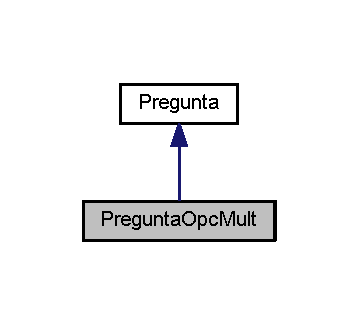
\includegraphics[width=172pt]{class_pregunta_opc_mult__inherit__graph}
\end{center}
\end{figure}


Collaboration diagram for Pregunta\-Opc\-Mult\-:\nopagebreak
\begin{figure}[H]
\begin{center}
\leavevmode
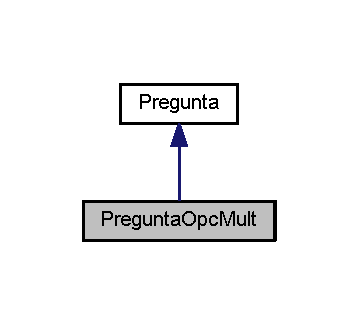
\includegraphics[width=172pt]{class_pregunta_opc_mult__coll__graph}
\end{center}
\end{figure}
\subsection*{Public Member Functions}
\begin{DoxyCompactItemize}
\item 
{\bf Pregunta\-Opc\-Mult} (std\-::string, std\-::string)
\item 
{\bf $\sim$\-Pregunta\-Opc\-Mult} ()
\item 
void {\bf responder} ()
\item 
void {\bf imprimir\-Pregunta} ()
\end{DoxyCompactItemize}
\subsection*{Private Attributes}
\begin{DoxyCompactItemize}
\item 
int {\bf numero\-Opciones}
\item 
std\-::vector$<$ std\-::string $>$ {\bf opcions}
\end{DoxyCompactItemize}
\subsection*{Additional Inherited Members}


\subsection{Detailed Description}


Definition at line 30 of file Preguntas.\-h.



\subsection{Constructor \& Destructor Documentation}
\index{Pregunta\-Opc\-Mult@{Pregunta\-Opc\-Mult}!Pregunta\-Opc\-Mult@{Pregunta\-Opc\-Mult}}
\index{Pregunta\-Opc\-Mult@{Pregunta\-Opc\-Mult}!PreguntaOpcMult@{Pregunta\-Opc\-Mult}}
\subsubsection[{Pregunta\-Opc\-Mult}]{\setlength{\rightskip}{0pt plus 5cm}Pregunta\-Opc\-Mult\-::\-Pregunta\-Opc\-Mult (
\begin{DoxyParamCaption}
\item[{std\-::string}]{input, }
\item[{std\-::string}]{opci}
\end{DoxyParamCaption}
)}\label{class_pregunta_opc_mult_a1da96a9953f5f8dae50114edb06ff23e}


Definition at line 72 of file Preguntas.\-cpp.


\begin{DoxyCode}
72                                                                 : Pregunta(input)
73 \{
74     \textcolor{comment}{//opciones=opci;}
75     \textcolor{keywordtype}{size\_t} noOpc;
76     numeroOpciones=0;
77     \textcolor{keywordtype}{string} container=\textcolor{stringliteral}{""};
78     \textcolor{keywordflow}{for} (noOpc=0;noOpc<opci.length();noOpc++)
79     \{
80         \textcolor{keywordflow}{if} (opci[noOpc]==\textcolor{charliteral}{'\(\backslash\)t'} || noOpc==(opci.length()-1))
81         \{
82             numeroOpciones++;
83             opcions.push\_back(container);
84             container=\textcolor{stringliteral}{""};
85             \textcolor{keywordflow}{continue};
86         \}
87         container+=opci[noOpc];
88     \}
89     \textcolor{comment}{//cout<<opci.length()<<"lasopcios\(\backslash\)n";}
90     \textcolor{comment}{//numeroOpciones=opci.length();}
91 \}
\end{DoxyCode}
\index{Pregunta\-Opc\-Mult@{Pregunta\-Opc\-Mult}!$\sim$\-Pregunta\-Opc\-Mult@{$\sim$\-Pregunta\-Opc\-Mult}}
\index{$\sim$\-Pregunta\-Opc\-Mult@{$\sim$\-Pregunta\-Opc\-Mult}!PreguntaOpcMult@{Pregunta\-Opc\-Mult}}
\subsubsection[{$\sim$\-Pregunta\-Opc\-Mult}]{\setlength{\rightskip}{0pt plus 5cm}Pregunta\-Opc\-Mult\-::$\sim$\-Pregunta\-Opc\-Mult (
\begin{DoxyParamCaption}
{}
\end{DoxyParamCaption}
)\hspace{0.3cm}{\ttfamily [inline]}}\label{class_pregunta_opc_mult_a533a24f45ccef0aed14aea03b0d7b85f}


Definition at line 34 of file Preguntas.\-h.


\begin{DoxyCode}
34 \{\};
\end{DoxyCode}


\subsection{Member Function Documentation}
\index{Pregunta\-Opc\-Mult@{Pregunta\-Opc\-Mult}!imprimir\-Pregunta@{imprimir\-Pregunta}}
\index{imprimir\-Pregunta@{imprimir\-Pregunta}!PreguntaOpcMult@{Pregunta\-Opc\-Mult}}
\subsubsection[{imprimir\-Pregunta}]{\setlength{\rightskip}{0pt plus 5cm}void Pregunta\-Opc\-Mult\-::imprimir\-Pregunta (
\begin{DoxyParamCaption}
{}
\end{DoxyParamCaption}
)\hspace{0.3cm}{\ttfamily [virtual]}}\label{class_pregunta_opc_mult_a2c87b73c52b7f65956f4a3bcb55ac719}


Reimplemented from {\bf Pregunta} \doxyref{}{p.}{class_pregunta_ac97860f3cd3d11c415e8cde6e529d7b9}.



Definition at line 114 of file Preguntas.\-cpp.


\begin{DoxyCode}
115 \{
116     \_\_super::imprimirPregunta();
117     cout<<endl;
118 
119     \textcolor{keywordflow}{for} (\textcolor{keywordtype}{int} i=0;i<numeroOpciones;i++)
120     \{
121         cout<<char(i+97)<<\textcolor{stringliteral}{") "}<<opcions[i]<<\textcolor{stringliteral}{"\(\backslash\)t"};
122     \}
123     cout<<\textcolor{stringliteral}{"\(\backslash\)n\(\backslash\)n"};
124 \}
\end{DoxyCode}
\index{Pregunta\-Opc\-Mult@{Pregunta\-Opc\-Mult}!responder@{responder}}
\index{responder@{responder}!PreguntaOpcMult@{Pregunta\-Opc\-Mult}}
\subsubsection[{responder}]{\setlength{\rightskip}{0pt plus 5cm}void Pregunta\-Opc\-Mult\-::responder (
\begin{DoxyParamCaption}
{}
\end{DoxyParamCaption}
)\hspace{0.3cm}{\ttfamily [virtual]}}\label{class_pregunta_opc_mult_aaae8febba0ce55b1b2682c8093f6b594}


Reimplemented from {\bf Pregunta} \doxyref{}{p.}{class_pregunta_aaf28e3a833e98b6b8bbd9267311a1ad2}.



Definition at line 93 of file Preguntas.\-cpp.


\begin{DoxyCode}
94 \{
95     \textcolor{keywordtype}{string} opciones=\textcolor{stringliteral}{""};
96     \textcolor{keywordflow}{for} (\textcolor{keywordtype}{int} j = 0; j < numeroOpciones; j++)
97     \{
98         opciones+=char(j+97);
99     \}
100     \textcolor{keywordtype}{char} opc = \_getch();
101     \textcolor{keywordflow}{for} (\textcolor{keywordtype}{unsigned} \textcolor{keywordtype}{int} i=0;i<opciones.length();i++)
102     \{
103         \textcolor{keywordflow}{if} (opciones[i] == opc)
104         \{
105             respuesta[0]=opc;
106             \textcolor{keywordflow}{return};
107         \}
108         
109     \}
110     responder();
111     
112 \}
\end{DoxyCode}


\subsection{Member Data Documentation}
\index{Pregunta\-Opc\-Mult@{Pregunta\-Opc\-Mult}!numero\-Opciones@{numero\-Opciones}}
\index{numero\-Opciones@{numero\-Opciones}!PreguntaOpcMult@{Pregunta\-Opc\-Mult}}
\subsubsection[{numero\-Opciones}]{\setlength{\rightskip}{0pt plus 5cm}int Pregunta\-Opc\-Mult\-::numero\-Opciones\hspace{0.3cm}{\ttfamily [private]}}\label{class_pregunta_opc_mult_a7648418e8001cb4d393a90bc301dd347}


Definition at line 39 of file Preguntas.\-h.

\index{Pregunta\-Opc\-Mult@{Pregunta\-Opc\-Mult}!opcions@{opcions}}
\index{opcions@{opcions}!PreguntaOpcMult@{Pregunta\-Opc\-Mult}}
\subsubsection[{opcions}]{\setlength{\rightskip}{0pt plus 5cm}std\-::vector$<$std\-::string$>$ Pregunta\-Opc\-Mult\-::opcions\hspace{0.3cm}{\ttfamily [private]}}\label{class_pregunta_opc_mult_a1a0c122cc9817d264f531e28b6e52a36}


Definition at line 40 of file Preguntas.\-h.



The documentation for this class was generated from the following files\-:\begin{DoxyCompactItemize}
\item 
Proyecto\-Integrador2/{\bf Preguntas.\-h}\item 
Proyecto\-Integrador2/{\bf Preguntas.\-cpp}\end{DoxyCompactItemize}

\section{Referencia de la Clase Validador}
\label{class_validador}\index{Validador@{Validador}}


{\ttfamily \#include $<$Encriptador.\-h$>$}

\subsection*{Métodos públicos}
\begin{DoxyCompactItemize}
\item 
{\bf Validador} (std\-::string filename)
\item 
{\bf $\sim$\-Validador} ()
\item 
bool {\bf es\-Valido} (std\-::string input)
\item 
std\-::string {\bf get\-Content} ()
\end{DoxyCompactItemize}
\subsection*{Atributos públicos}
\begin{DoxyCompactItemize}
\item 
std\-::string {\bf path}
\item 
int {\bf size}
\end{DoxyCompactItemize}


\subsection{Descripción detallada}


Definición en la línea 31 del archivo Encriptador.\-h.



\subsection{Documentación del constructor y destructor}
\index{Validador@{Validador}!Validador@{Validador}}
\index{Validador@{Validador}!Validador@{Validador}}
\subsubsection[{Validador}]{\setlength{\rightskip}{0pt plus 5cm}Validador\-::\-Validador (
\begin{DoxyParamCaption}
\item[{std\-::string}]{filename}
\end{DoxyParamCaption}
)}\label{class_validador_ab2626f57c35c5349a142c9b8a82ec5de}


Definición en la línea 86 del archivo Encriptador.\-cpp.


\begin{DoxyCode}
87 \{
88     \textcolor{keywordflow}{for} (\textcolor{keywordtype}{char} i=\textcolor{charliteral}{'A'};i<=\textcolor{charliteral}{'Z'};i++)
89     \{
90         \textcolor{comment}{//std::cout<<i<<std::endl;}
91         std::string tmpcontent;
92         path = \textcolor{stringliteral}{"N:\(\backslash\)\(\backslash\)"}+filename;
93         path[0]=i;
94         \textcolor{comment}{//std::cout<<"Checando en "+path<<std::endl;}
95         std::ifstream archivoClave (path, std::ifstream::binary);
96         \textcolor{keywordflow}{if} (archivoClave.is\_open())
97         \{
98 
99             content.assign( (std::istreambuf\_iterator<char>(archivoClave) ),
100                 (std::istreambuf\_iterator<char>()    ) );
101             \textcolor{keywordflow}{break};
102             tmpcontent.assign(content.data());
103         \}
104 
105         \textcolor{comment}{//std::cout<<tmpcontent<<std::endl;}
106 
107     \}
108 \}
\end{DoxyCode}
\index{Validador@{Validador}!$\sim$\-Validador@{$\sim$\-Validador}}
\index{$\sim$\-Validador@{$\sim$\-Validador}!Validador@{Validador}}
\subsubsection[{$\sim$\-Validador}]{\setlength{\rightskip}{0pt plus 5cm}Validador\-::$\sim$\-Validador (
\begin{DoxyParamCaption}
{}
\end{DoxyParamCaption}
)}\label{class_validador_ab10f475fc21b063297ea9e88ecc248c1}


Definición en la línea 81 del archivo Encriptador.\-cpp.


\begin{DoxyCode}
82 \{
83 
84 \}
\end{DoxyCode}


\subsection{Documentación de las funciones miembro}
\index{Validador@{Validador}!es\-Valido@{es\-Valido}}
\index{es\-Valido@{es\-Valido}!Validador@{Validador}}
\subsubsection[{es\-Valido}]{\setlength{\rightskip}{0pt plus 5cm}bool Validador\-::es\-Valido (
\begin{DoxyParamCaption}
\item[{std\-::string}]{input}
\end{DoxyParamCaption}
)}\label{class_validador_aa28aeee63d24ac104492eac4a24ef215}


Definición en la línea 68 del archivo Encriptador.\-cpp.


\begin{DoxyCode}
69 \{
70     std::string contenido = getContent();
71     \textcolor{keywordflow}{if} (input == contenido)
72     \{
73         \textcolor{keywordflow}{return} \textcolor{keyword}{true};
74     \} 
75     \textcolor{keywordflow}{else}
76     \{
77         \textcolor{keywordflow}{return} \textcolor{keyword}{false};
78     \}
79 \}
\end{DoxyCode}


Gráfico de llamadas para esta función\-:
\nopagebreak
\begin{figure}[H]
\begin{center}
\leavevmode
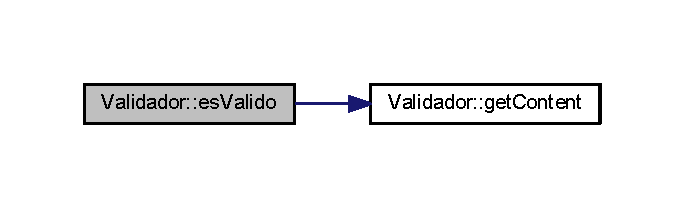
\includegraphics[width=328pt]{class_validador_aa28aeee63d24ac104492eac4a24ef215_cgraph}
\end{center}
\end{figure}




Gráfico de llamadas a esta función\-:
\nopagebreak
\begin{figure}[H]
\begin{center}
\leavevmode
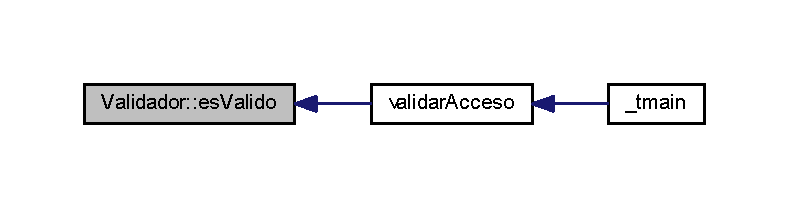
\includegraphics[width=350pt]{class_validador_aa28aeee63d24ac104492eac4a24ef215_icgraph}
\end{center}
\end{figure}


\index{Validador@{Validador}!get\-Content@{get\-Content}}
\index{get\-Content@{get\-Content}!Validador@{Validador}}
\subsubsection[{get\-Content}]{\setlength{\rightskip}{0pt plus 5cm}std\-::string Validador\-::get\-Content (
\begin{DoxyParamCaption}
{}
\end{DoxyParamCaption}
)}\label{class_validador_af37049c367add17c5f52e938608251f5}


Definición en la línea 63 del archivo Encriptador.\-cpp.


\begin{DoxyCode}
64 \{
65     \textcolor{keywordflow}{return} content;
66 \}
\end{DoxyCode}


Gráfico de llamadas a esta función\-:
\nopagebreak
\begin{figure}[H]
\begin{center}
\leavevmode
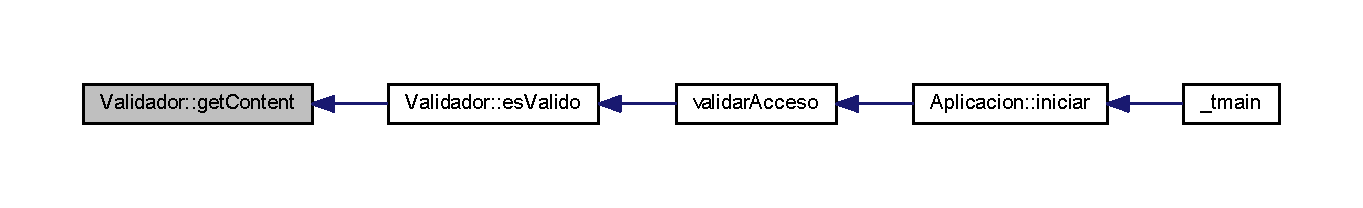
\includegraphics[width=350pt]{class_validador_af37049c367add17c5f52e938608251f5_icgraph}
\end{center}
\end{figure}




\subsection{Documentación de los datos miembro}
\index{Validador@{Validador}!path@{path}}
\index{path@{path}!Validador@{Validador}}
\subsubsection[{path}]{\setlength{\rightskip}{0pt plus 5cm}std\-::string Validador\-::path}\label{class_validador_a55da861f4a63a702a554f4b0f4834749}


Definición en la línea 37 del archivo Encriptador.\-h.

\index{Validador@{Validador}!size@{size}}
\index{size@{size}!Validador@{Validador}}
\subsubsection[{size}]{\setlength{\rightskip}{0pt plus 5cm}int Validador\-::size}\label{class_validador_a34374bc7f9d8ffac55db94a6325e41bd}


Definición en la línea 38 del archivo Encriptador.\-h.



La documentación para esta clase fue generada a partir de los siguientes ficheros\-:\begin{DoxyCompactItemize}
\item 
Proyecto\-Integrador2/{\bf Encriptador.\-h}\item 
Proyecto\-Integrador2/{\bf Encriptador.\-cpp}\end{DoxyCompactItemize}

\chapter{File Documentation}
\section{Proyecto\-Integrador2/\-Aplicacion.cpp File Reference}
\label{_aplicacion_8cpp}\index{Proyecto\-Integrador2/\-Aplicacion.\-cpp@{Proyecto\-Integrador2/\-Aplicacion.\-cpp}}
{\ttfamily \#include \char`\"{}stdafx.\-h\char`\"{}}\\*
{\ttfamily \#include $<$thread$>$}\\*
{\ttfamily \#include $<$iostream$>$}\\*
{\ttfamily \#include $<$chrono$>$}\\*
{\ttfamily \#include \char`\"{}Encriptador.\-h\char`\"{}}\\*
{\ttfamily \#include \char`\"{}Preguntas.\-h\char`\"{}}\\*
{\ttfamily \#include \char`\"{}Cuestionario.\-h\char`\"{}}\\*
{\ttfamily \#include \char`\"{}Consulta.\-h\char`\"{}}\\*
{\ttfamily \#include \char`\"{}Aplicacion.\-h\char`\"{}}\\*
{\ttfamily \#include \char`\"{}Menu.\-h\char`\"{}}\\*
Include dependency graph for Aplicacion.\-cpp\-:\nopagebreak
\begin{figure}[H]
\begin{center}
\leavevmode
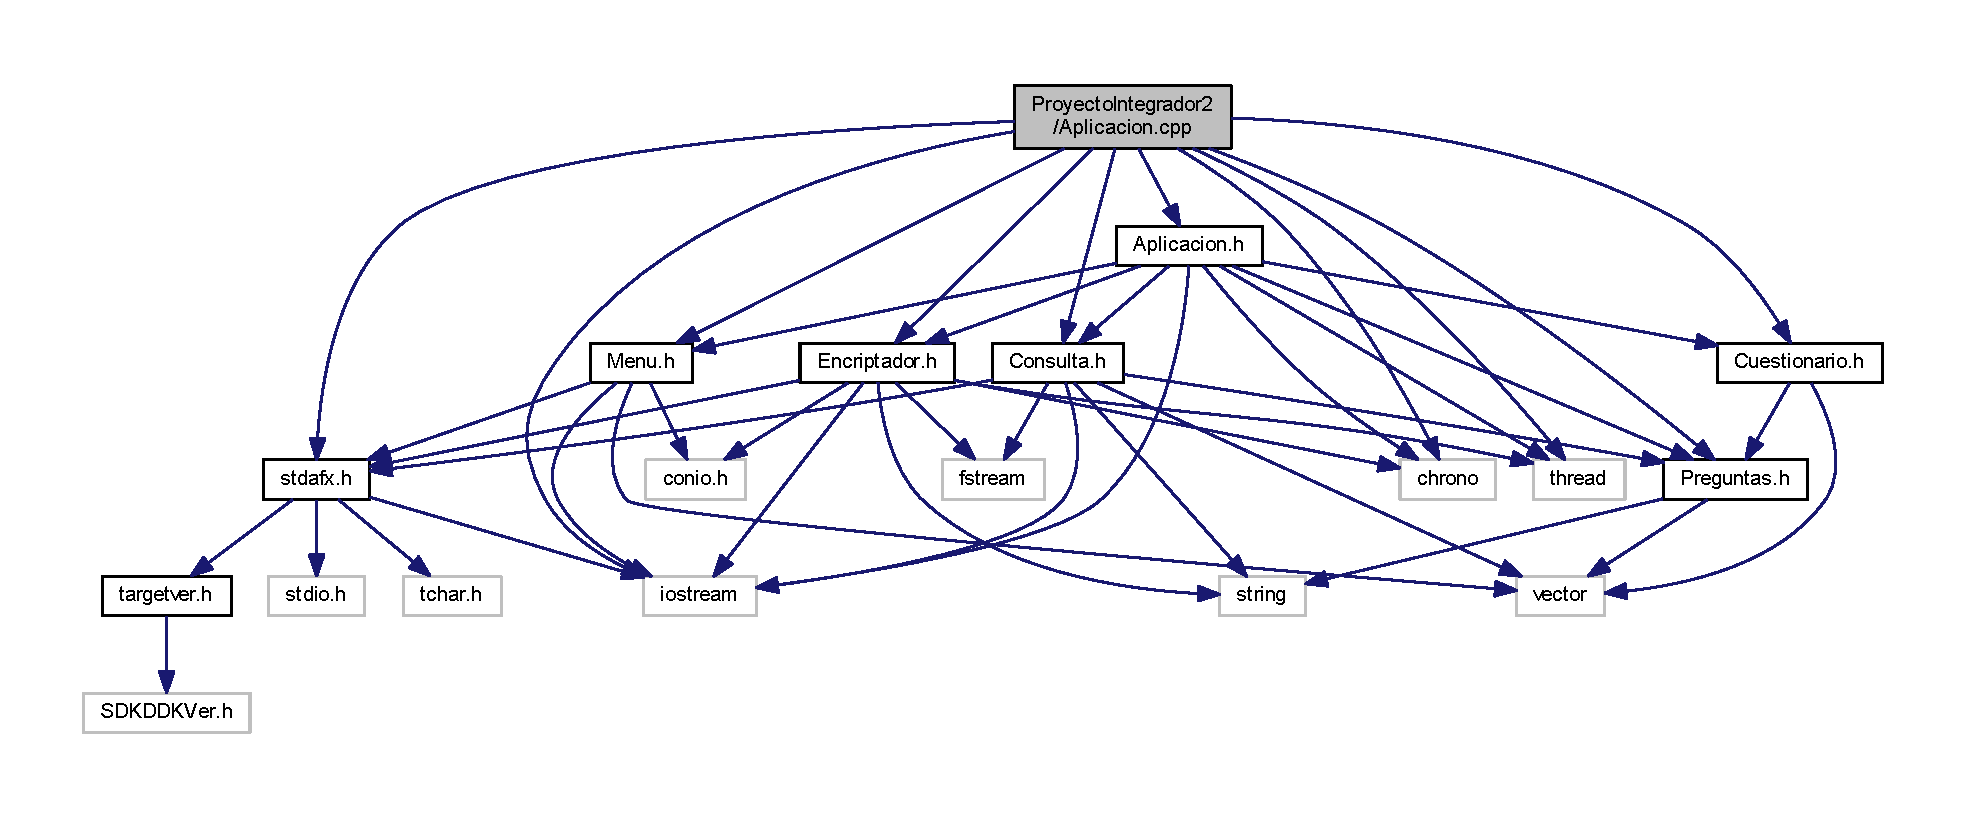
\includegraphics[width=350pt]{_aplicacion_8cpp__incl}
\end{center}
\end{figure}

\section{Proyecto\-Integrador2/\-Aplicacion.h File Reference}
\label{_aplicacion_8h}\index{Proyecto\-Integrador2/\-Aplicacion.\-h@{Proyecto\-Integrador2/\-Aplicacion.\-h}}
{\ttfamily \#include $<$thread$>$}\\*
{\ttfamily \#include $<$iostream$>$}\\*
{\ttfamily \#include $<$chrono$>$}\\*
{\ttfamily \#include \char`\"{}Encriptador.\-h\char`\"{}}\\*
{\ttfamily \#include \char`\"{}Preguntas.\-h\char`\"{}}\\*
{\ttfamily \#include \char`\"{}Cuestionario.\-h\char`\"{}}\\*
{\ttfamily \#include \char`\"{}Consulta.\-h\char`\"{}}\\*
{\ttfamily \#include \char`\"{}Menu.\-h\char`\"{}}\\*
Include dependency graph for Aplicacion.\-h\-:\nopagebreak
\begin{figure}[H]
\begin{center}
\leavevmode
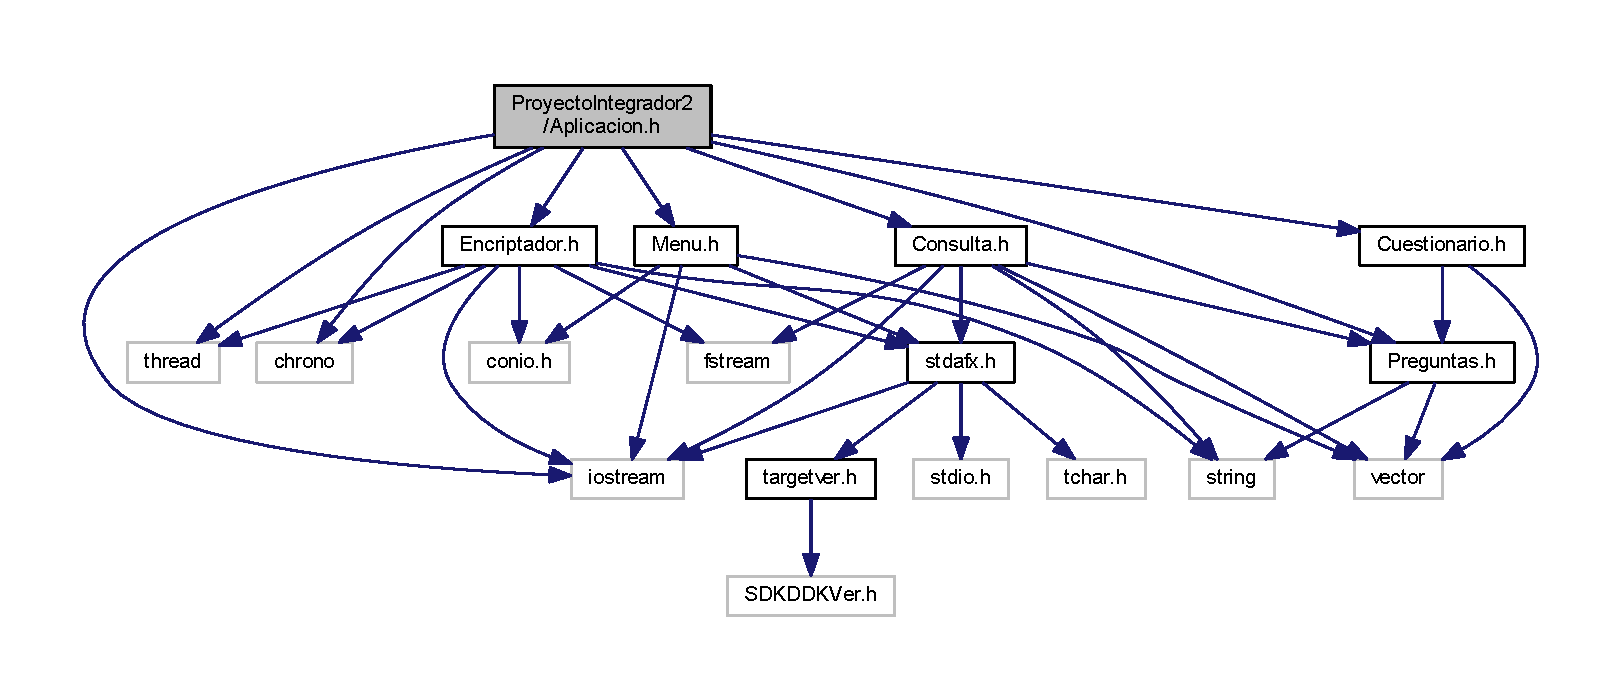
\includegraphics[width=350pt]{_aplicacion_8h__incl}
\end{center}
\end{figure}
This graph shows which files directly or indirectly include this file\-:\nopagebreak
\begin{figure}[H]
\begin{center}
\leavevmode
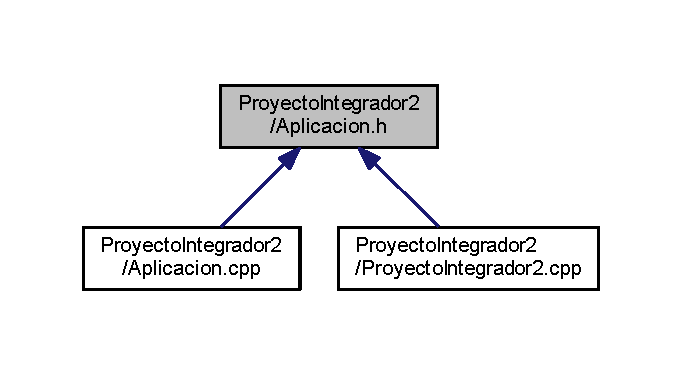
\includegraphics[width=327pt]{_aplicacion_8h__dep__incl}
\end{center}
\end{figure}
\subsection*{Classes}
\begin{DoxyCompactItemize}
\item 
class {\bf Aplicacion}
\end{DoxyCompactItemize}

\section{Proyecto\-Integrador2/\-Consulta.cpp File Reference}
\label{_consulta_8cpp}\index{Proyecto\-Integrador2/\-Consulta.\-cpp@{Proyecto\-Integrador2/\-Consulta.\-cpp}}
{\ttfamily \#include \char`\"{}stdafx.\-h\char`\"{}}\\*
{\ttfamily \#include $<$string$>$}\\*
{\ttfamily \#include $<$iostream$>$}\\*
{\ttfamily \#include $<$fstream$>$}\\*
{\ttfamily \#include $<$vector$>$}\\*
{\ttfamily \#include \char`\"{}Preguntas.\-h\char`\"{}}\\*
{\ttfamily \#include \char`\"{}Consulta.\-h\char`\"{}}\\*
Include dependency graph for Consulta.\-cpp\-:\nopagebreak
\begin{figure}[H]
\begin{center}
\leavevmode
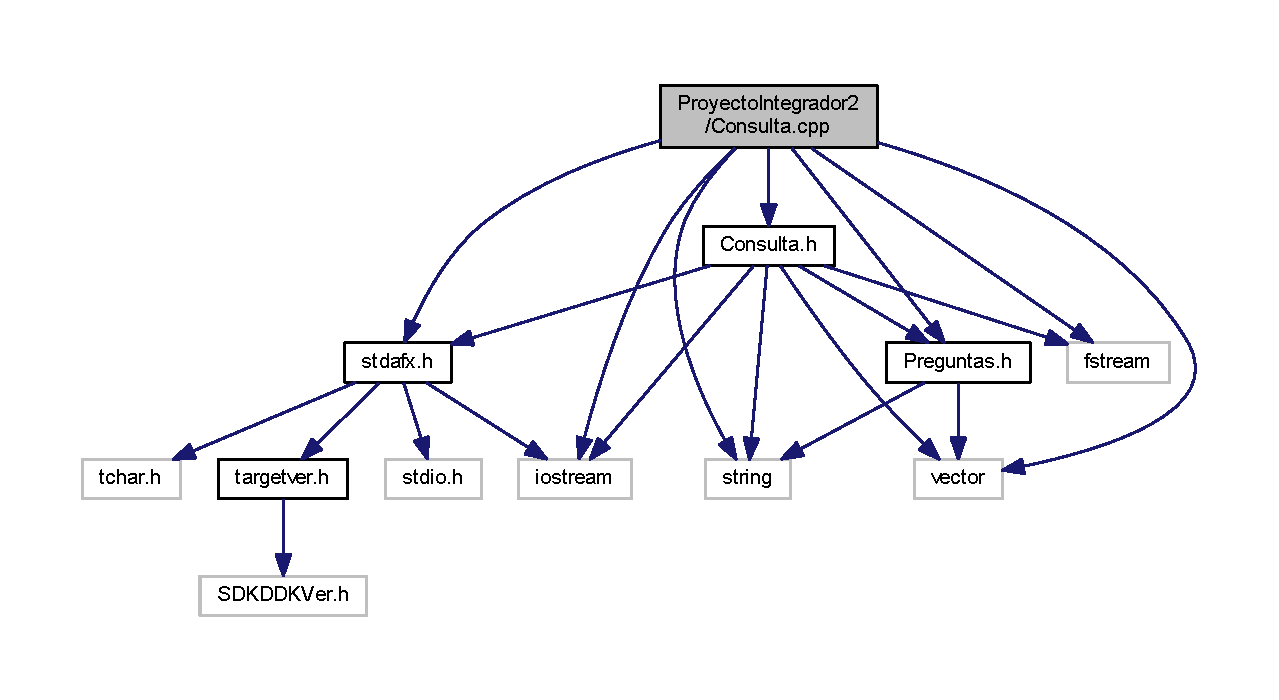
\includegraphics[width=350pt]{_consulta_8cpp__incl}
\end{center}
\end{figure}

\section{Proyecto\-Integrador2/\-Consulta.h File Reference}
\label{_consulta_8h}\index{Proyecto\-Integrador2/\-Consulta.\-h@{Proyecto\-Integrador2/\-Consulta.\-h}}
{\ttfamily \#include \char`\"{}stdafx.\-h\char`\"{}}\\*
{\ttfamily \#include $<$string$>$}\\*
{\ttfamily \#include $<$iostream$>$}\\*
{\ttfamily \#include $<$fstream$>$}\\*
{\ttfamily \#include $<$vector$>$}\\*
{\ttfamily \#include \char`\"{}Preguntas.\-h\char`\"{}}\\*
Include dependency graph for Consulta.\-h\-:\nopagebreak
\begin{figure}[H]
\begin{center}
\leavevmode
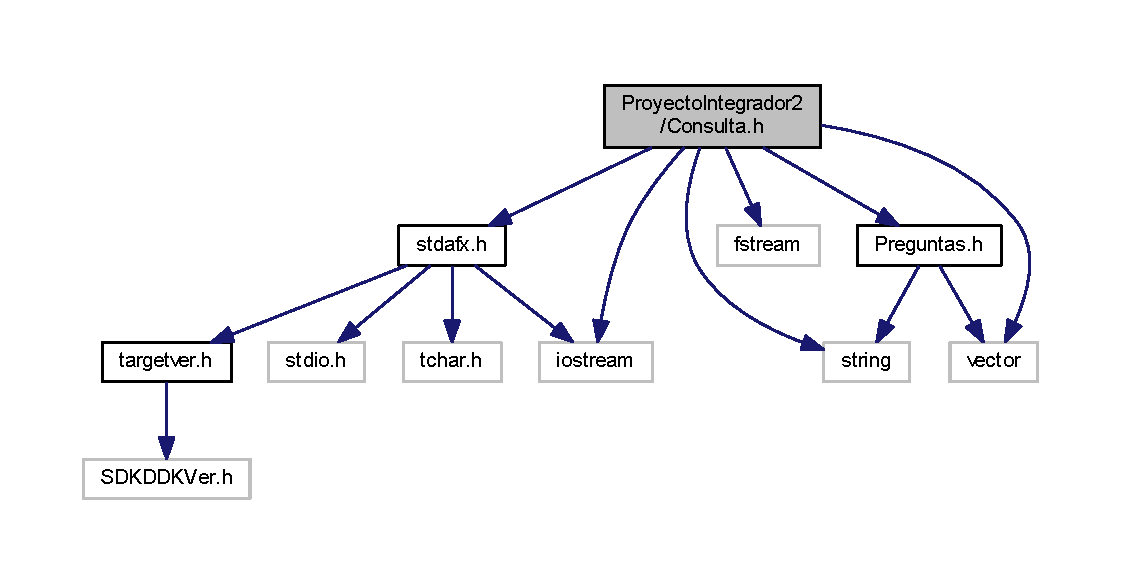
\includegraphics[width=350pt]{_consulta_8h__incl}
\end{center}
\end{figure}
This graph shows which files directly or indirectly include this file\-:\nopagebreak
\begin{figure}[H]
\begin{center}
\leavevmode
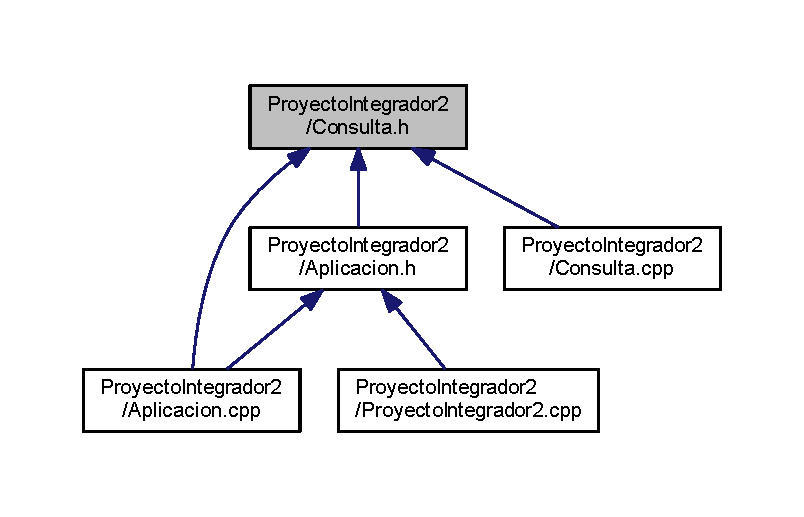
\includegraphics[width=350pt]{_consulta_8h__dep__incl}
\end{center}
\end{figure}
\subsection*{Classes}
\begin{DoxyCompactItemize}
\item 
class {\bf Consulta}
\end{DoxyCompactItemize}

\section{Proyecto\-Integrador2/\-Cuestionario.cpp File Reference}
\label{_cuestionario_8cpp}\index{Proyecto\-Integrador2/\-Cuestionario.\-cpp@{Proyecto\-Integrador2/\-Cuestionario.\-cpp}}
{\ttfamily \#include \char`\"{}stdafx.\-h\char`\"{}}\\*
{\ttfamily \#include \char`\"{}Cuestionario.\-h\char`\"{}}\\*
{\ttfamily \#include \char`\"{}Preguntas.\-h\char`\"{}}\\*
{\ttfamily \#include $<$vector$>$}\\*
{\ttfamily \#include $<$fstream$>$}\\*
{\ttfamily \#include $<$chrono$>$}\\*
{\ttfamily \#include $<$ctime$>$}\\*
{\ttfamily \#include $<$sstream$>$}\\*
Include dependency graph for Cuestionario.\-cpp\-:\nopagebreak
\begin{figure}[H]
\begin{center}
\leavevmode
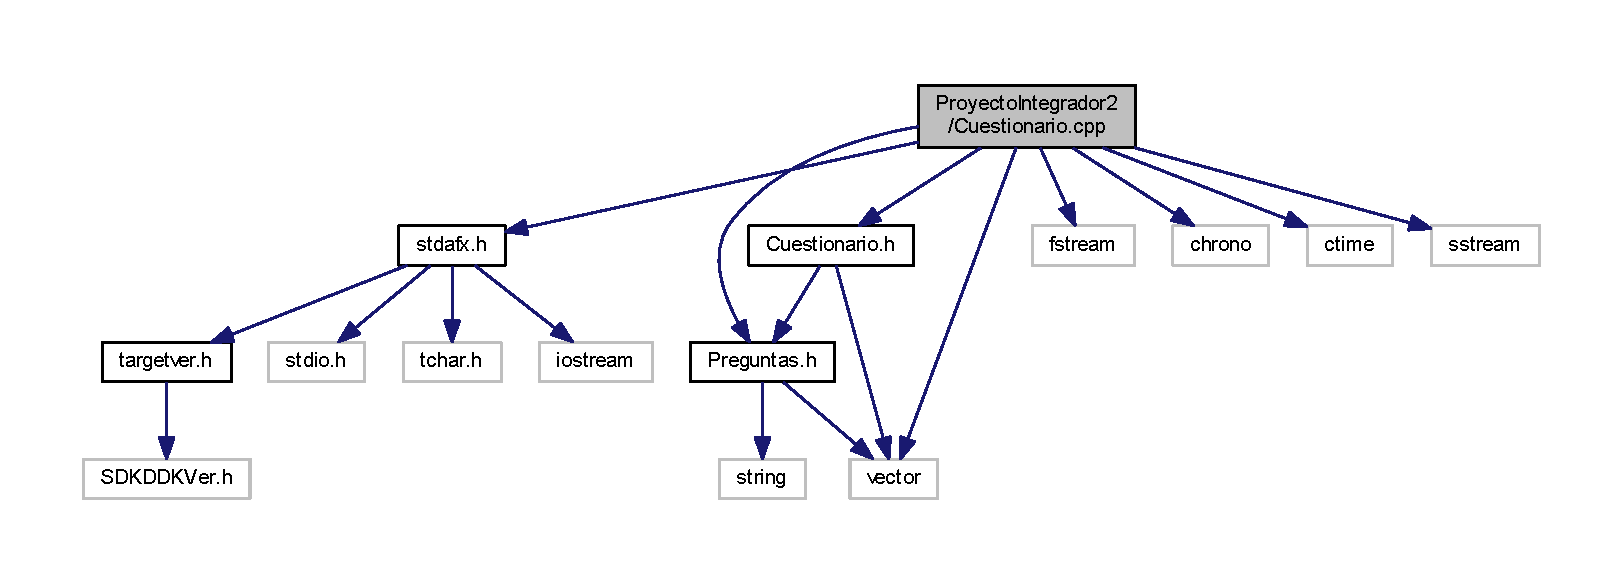
\includegraphics[width=350pt]{_cuestionario_8cpp__incl}
\end{center}
\end{figure}

\section{Referencia del Archivo Proyecto\-Integrador2/\-Cuestionario.h}
\label{_cuestionario_8h}\index{Proyecto\-Integrador2/\-Cuestionario.\-h@{Proyecto\-Integrador2/\-Cuestionario.\-h}}
{\ttfamily \#include \char`\"{}Preguntas.\-h\char`\"{}}\\*
{\ttfamily \#include $<$vector$>$}\\*
Dependencia gráfica adjunta para Cuestionario.\-h\-:
\nopagebreak
\begin{figure}[H]
\begin{center}
\leavevmode
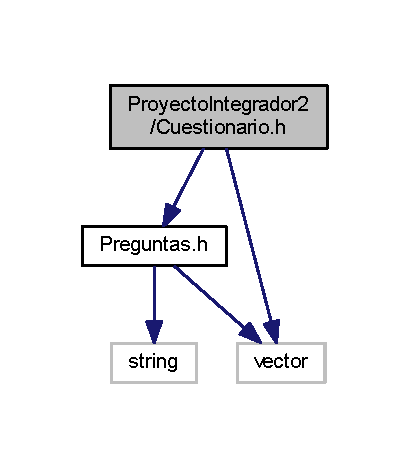
\includegraphics[width=197pt]{_cuestionario_8h__incl}
\end{center}
\end{figure}
Gráfico de los archivos que directa o indirectamente incluyen a este archivo\-:
\nopagebreak
\begin{figure}[H]
\begin{center}
\leavevmode
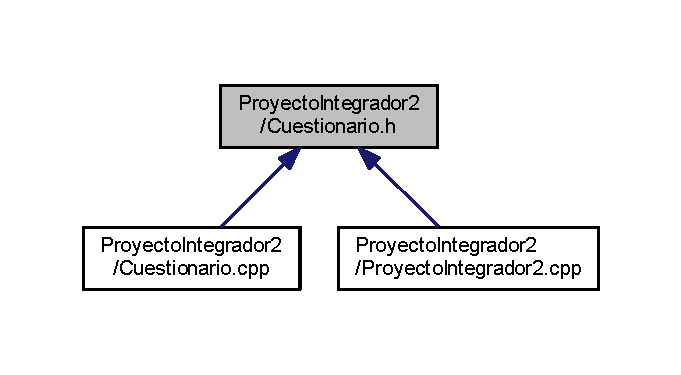
\includegraphics[width=327pt]{_cuestionario_8h__dep__incl}
\end{center}
\end{figure}
\subsection*{Clases}
\begin{DoxyCompactItemize}
\item 
class {\bf Cuestionario}
\end{DoxyCompactItemize}

\section{Proyecto\-Integrador2/\-Encriptador.cpp File Reference}
\label{_encriptador_8cpp}\index{Proyecto\-Integrador2/\-Encriptador.\-cpp@{Proyecto\-Integrador2/\-Encriptador.\-cpp}}
{\ttfamily \#include \char`\"{}stdafx.\-h\char`\"{}}\\*
{\ttfamily \#include $<$thread$>$}\\*
{\ttfamily \#include $<$string$>$}\\*
{\ttfamily \#include $<$iostream$>$}\\*
{\ttfamily \#include $<$fstream$>$}\\*
{\ttfamily \#include $<$conio.\-h$>$}\\*
{\ttfamily \#include $<$chrono$>$}\\*
{\ttfamily \#include \char`\"{}Encriptador.\-h\char`\"{}}\\*
Include dependency graph for Encriptador.\-cpp\-:\nopagebreak
\begin{figure}[H]
\begin{center}
\leavevmode
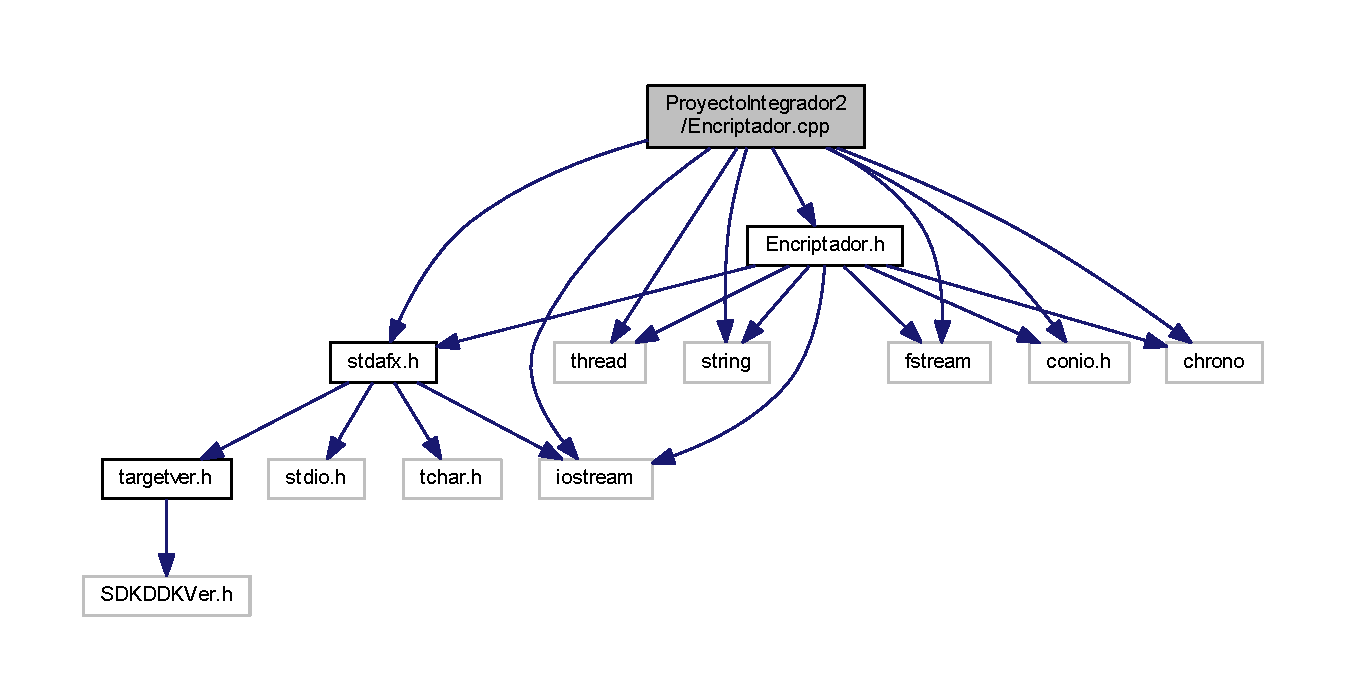
\includegraphics[width=350pt]{_encriptador_8cpp__incl}
\end{center}
\end{figure}
\subsection*{Functions}
\begin{DoxyCompactItemize}
\item 
bool {\bf validar\-Acceso} ()
\end{DoxyCompactItemize}


\subsection{Function Documentation}
\index{Encriptador.\-cpp@{Encriptador.\-cpp}!validar\-Acceso@{validar\-Acceso}}
\index{validar\-Acceso@{validar\-Acceso}!Encriptador.cpp@{Encriptador.\-cpp}}
\subsubsection[{validar\-Acceso}]{\setlength{\rightskip}{0pt plus 5cm}bool validar\-Acceso (
\begin{DoxyParamCaption}
{}
\end{DoxyParamCaption}
)}\label{_encriptador_8cpp_a514eeb9d37c47513308d43f3ddcb5d66}


Definition at line 110 of file Encriptador.\-cpp.


\begin{DoxyCode}
111 \{
112     Encriptador crypt(\textcolor{stringliteral}{"RSeCDf23g4ihjlk6auvMLxpQUmAEBwzyFGontJHIqKr7 Ts8ON9PXVWZ0Y15bcd"}, \textcolor{stringliteral}{"
      abcdefghijklmnopqrstuvwxyzABCDEFGHIJKLMNOPQRSTUVWXYZ0123456789 "});
113     Validador valid(\textcolor{stringliteral}{"clave.bin"});
114     \textcolor{keywordtype}{string} clave = \textcolor{stringliteral}{"pablito clavo un clavito en la calva de un calvito"};
115     \textcolor{comment}{//cout<<"Buscando el archivo"<<endl;}
116     \textcolor{comment}{//if(valid.encontrado)cout<<"Archivo encontrado en " << valid.path<<endl;}
117     \textcolor{comment}{//cout<<crypt.Cifrar(clave)<<endl;}
118     \textcolor{keywordtype}{bool} validacion =valid.esValido(crypt.Cifrar(clave));
119     \textcolor{keywordflow}{if} (validacion)
120     \{
121         \textcolor{comment}{//      Acceso=true;}
122         \textcolor{comment}{//cout<<"Acceso Permitido"<<endl;}
123         \textcolor{keywordflow}{return} \textcolor{keyword}{true};
124     \}
125     \textcolor{keywordflow}{else}
126     \{
127         \textcolor{comment}{//      Acceso=false;}
128         cout<<\textcolor{stringliteral}{"Acceso Denegado"}<<endl;
129 
130         \textcolor{keywordflow}{return} \textcolor{keyword}{false};
131 
132     \}
133     \textcolor{comment}{//cout<<"Contenido del archivo: "<<valid.getContent()<<endl;}
134     \textcolor{comment}{//  cout<<"Contenido del archivo decifrado: " << crypt.Decifrar(valid.content)<<endl;}
135     \textcolor{comment}{//  cout<<"Clave correcta: " << clave<<endl;}
136 \}
\end{DoxyCode}


Here is the call graph for this function\-:\nopagebreak
\begin{figure}[H]
\begin{center}
\leavevmode
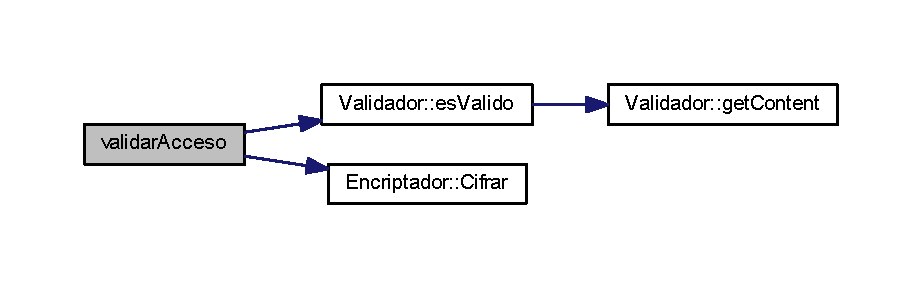
\includegraphics[width=350pt]{_encriptador_8cpp_a514eeb9d37c47513308d43f3ddcb5d66_cgraph}
\end{center}
\end{figure}




Here is the caller graph for this function\-:\nopagebreak
\begin{figure}[H]
\begin{center}
\leavevmode
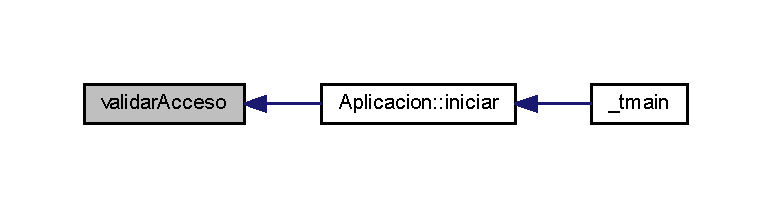
\includegraphics[width=350pt]{_encriptador_8cpp_a514eeb9d37c47513308d43f3ddcb5d66_icgraph}
\end{center}
\end{figure}



\section{Referencia del Archivo Proyecto\-Integrador2/\-Encriptador.h}
\label{_encriptador_8h}\index{Proyecto\-Integrador2/\-Encriptador.\-h@{Proyecto\-Integrador2/\-Encriptador.\-h}}
{\ttfamily \#include \char`\"{}stdafx.\-h\char`\"{}}\\*
{\ttfamily \#include $<$thread$>$}\\*
{\ttfamily \#include $<$string$>$}\\*
{\ttfamily \#include $<$iostream$>$}\\*
{\ttfamily \#include $<$fstream$>$}\\*
{\ttfamily \#include $<$conio.\-h$>$}\\*
{\ttfamily \#include $<$chrono$>$}\\*
Dependencia gráfica adjunta para Encriptador.\-h\-:
\nopagebreak
\begin{figure}[H]
\begin{center}
\leavevmode
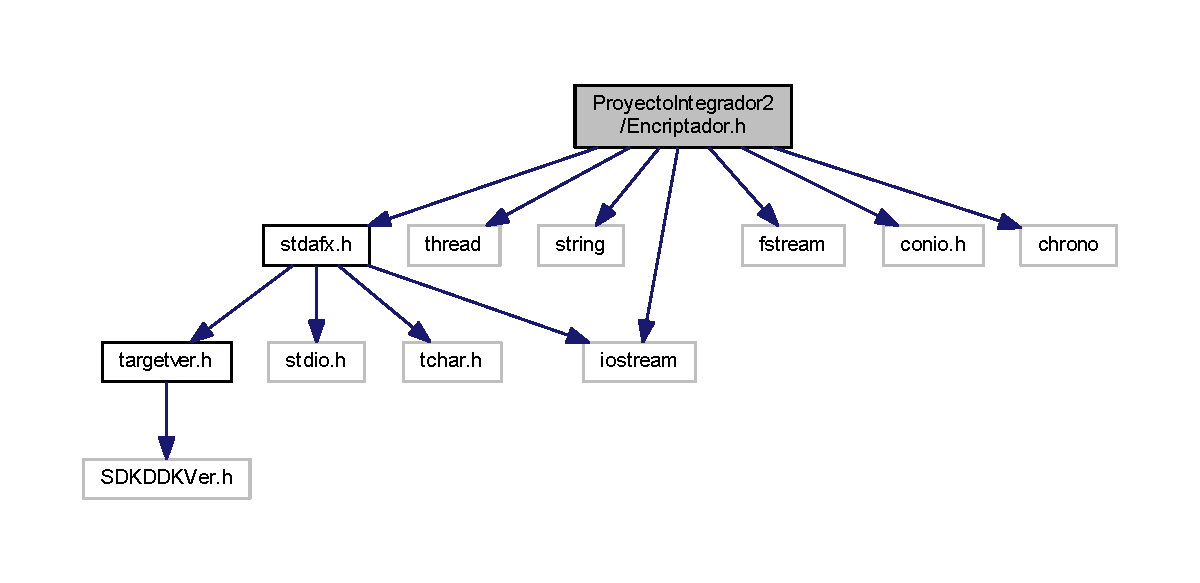
\includegraphics[width=350pt]{_encriptador_8h__incl}
\end{center}
\end{figure}
Gráfico de los archivos que directa o indirectamente incluyen a este archivo\-:
\nopagebreak
\begin{figure}[H]
\begin{center}
\leavevmode
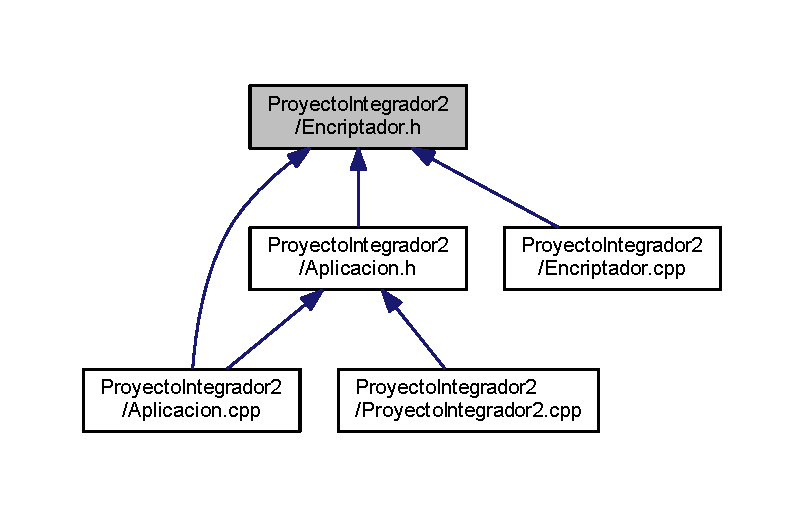
\includegraphics[width=327pt]{_encriptador_8h__dep__incl}
\end{center}
\end{figure}
\subsection*{Clases}
\begin{DoxyCompactItemize}
\item 
class {\bf Encriptador}
\item 
class {\bf Validador}
\end{DoxyCompactItemize}
\subsection*{Funciones}
\begin{DoxyCompactItemize}
\item 
bool {\bf validar\-Acceso} ()
\end{DoxyCompactItemize}


\subsection{Documentación de las funciones}
\index{Encriptador.\-h@{Encriptador.\-h}!validar\-Acceso@{validar\-Acceso}}
\index{validar\-Acceso@{validar\-Acceso}!Encriptador.h@{Encriptador.\-h}}
\subsubsection[{validar\-Acceso}]{\setlength{\rightskip}{0pt plus 5cm}bool validar\-Acceso (
\begin{DoxyParamCaption}
{}
\end{DoxyParamCaption}
)}\label{_encriptador_8h_a514eeb9d37c47513308d43f3ddcb5d66}


Definición en la línea 110 del archivo Encriptador.\-cpp.


\begin{DoxyCode}
111 \{
112     Encriptador crypt(\textcolor{stringliteral}{"RSeCDf23g4ihjlk6auvMLxpQUmAEBwzyFGontJHIqKr7 Ts8ON9PXVWZ0Y15bcd"}, \textcolor{stringliteral}{"
      abcdefghijklmnopqrstuvwxyzABCDEFGHIJKLMNOPQRSTUVWXYZ0123456789 "});
113     Validador valid(\textcolor{stringliteral}{"clave.txt"});
114     \textcolor{keywordtype}{string} clave = \textcolor{stringliteral}{"pablito clavo un clavito en la calva de un calvito"};
115     \textcolor{comment}{//cout<<"Buscando el archivo"<<endl;}
116     \textcolor{comment}{//if(valid.encontrado)cout<<"Archivo encontrado en " << valid.path<<endl;}
117     \textcolor{comment}{//cout<<crypt.Cifrar(clave)<<endl;}
118     \textcolor{keywordtype}{bool} validacion =valid.esValido(crypt.Cifrar(clave));
119     \textcolor{keywordflow}{if} (validacion)
120     \{
121         \textcolor{comment}{//      Acceso=true;}
122         \textcolor{comment}{//cout<<"Acceso Permitido"<<endl;}
123         \textcolor{keywordflow}{return} \textcolor{keyword}{true};
124     \}
125     \textcolor{keywordflow}{else}
126     \{
127         \textcolor{comment}{//      Acceso=false;}
128         cout<<\textcolor{stringliteral}{"Acceso Denegado"}<<endl;
129 
130         \textcolor{keywordflow}{return} \textcolor{keyword}{false};
131 
132     \}
133     \textcolor{comment}{//cout<<"Contenido del archivo: "<<valid.getContent()<<endl;}
134     \textcolor{comment}{//  cout<<"Contenido del archivo decifrado: " << crypt.Decifrar(valid.content)<<endl;}
135     \textcolor{comment}{//  cout<<"Clave correcta: " << clave<<endl;}
136 \}
\end{DoxyCode}


Gráfico de llamadas para esta función\-:
\nopagebreak
\begin{figure}[H]
\begin{center}
\leavevmode
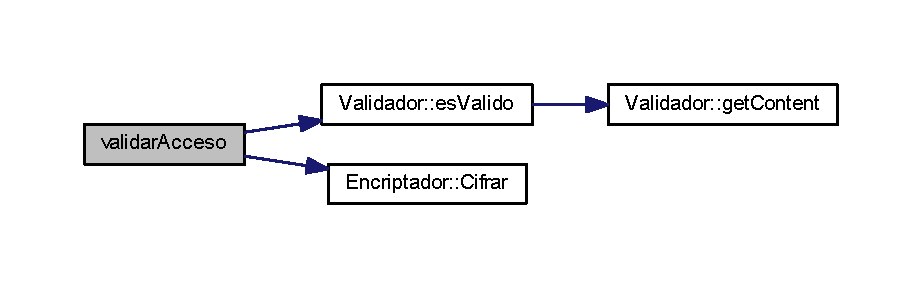
\includegraphics[width=350pt]{_encriptador_8h_a514eeb9d37c47513308d43f3ddcb5d66_cgraph}
\end{center}
\end{figure}




Gráfico de llamadas a esta función\-:
\nopagebreak
\begin{figure}[H]
\begin{center}
\leavevmode
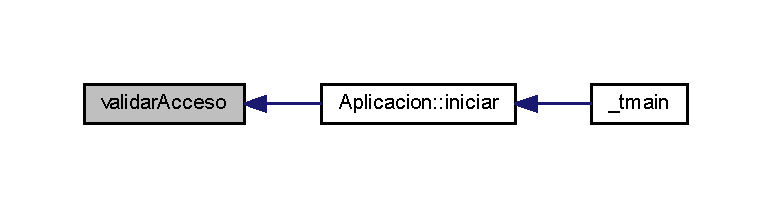
\includegraphics[width=240pt]{_encriptador_8h_a514eeb9d37c47513308d43f3ddcb5d66_icgraph}
\end{center}
\end{figure}



\section{Proyecto\-Integrador2/\-Menu.cpp File Reference}
\label{_menu_8cpp}\index{Proyecto\-Integrador2/\-Menu.\-cpp@{Proyecto\-Integrador2/\-Menu.\-cpp}}
{\ttfamily \#include \char`\"{}stdafx.\-h\char`\"{}}\\*
{\ttfamily \#include $<$iostream$>$}\\*
{\ttfamily \#include $<$vector$>$}\\*
{\ttfamily \#include $<$conio.\-h$>$}\\*
{\ttfamily \#include $<$string$>$}\\*
{\ttfamily \#include \char`\"{}Menu.\-h\char`\"{}}\\*
Include dependency graph for Menu.\-cpp\-:\nopagebreak
\begin{figure}[H]
\begin{center}
\leavevmode
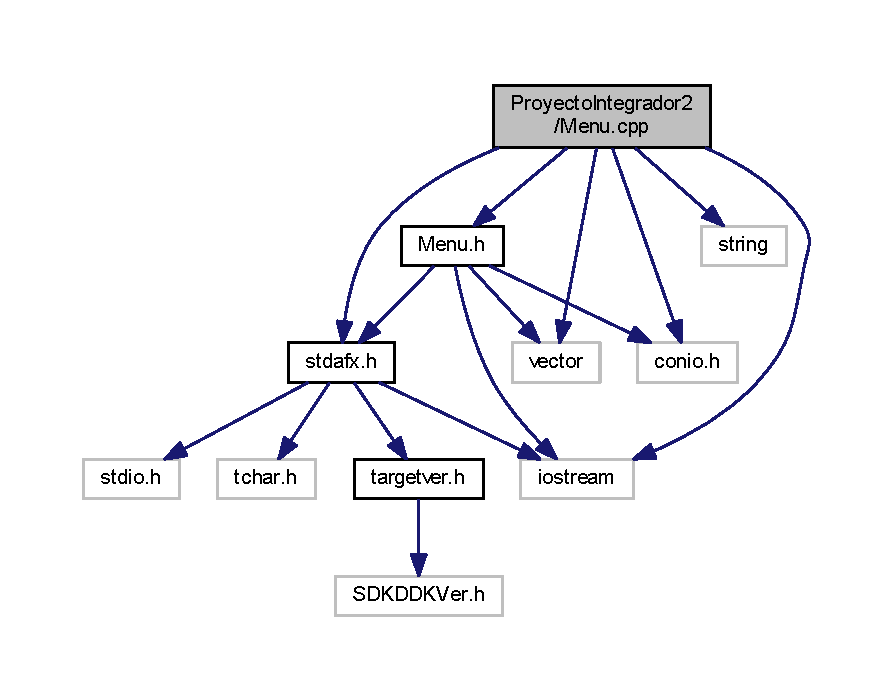
\includegraphics[width=350pt]{_menu_8cpp__incl}
\end{center}
\end{figure}

\section{Proyecto\-Integrador2/\-Menu.h File Reference}
\label{_menu_8h}\index{Proyecto\-Integrador2/\-Menu.\-h@{Proyecto\-Integrador2/\-Menu.\-h}}
{\ttfamily \#include \char`\"{}stdafx.\-h\char`\"{}}\\*
{\ttfamily \#include $<$iostream$>$}\\*
{\ttfamily \#include $<$vector$>$}\\*
{\ttfamily \#include $<$conio.\-h$>$}\\*
Include dependency graph for Menu.\-h\-:\nopagebreak
\begin{figure}[H]
\begin{center}
\leavevmode
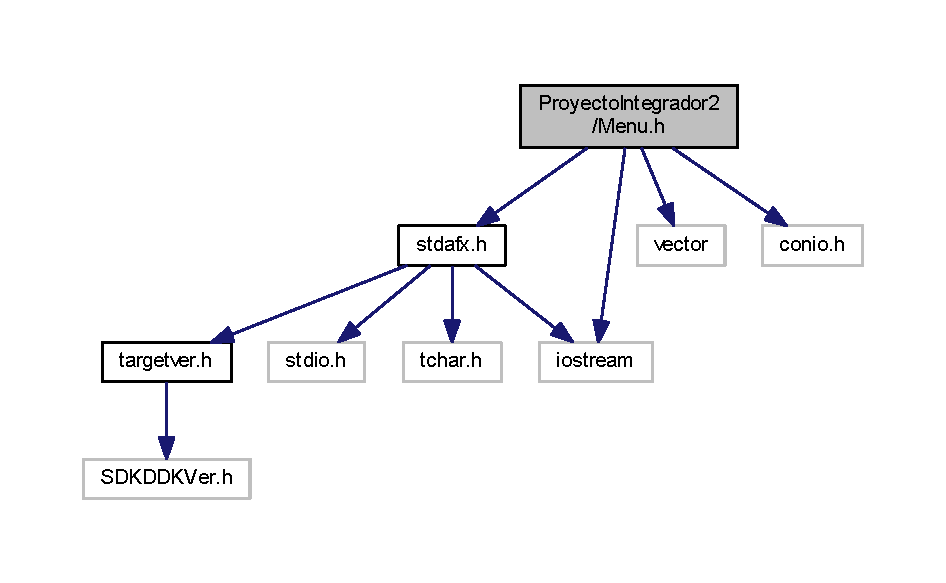
\includegraphics[width=350pt]{_menu_8h__incl}
\end{center}
\end{figure}
This graph shows which files directly or indirectly include this file\-:\nopagebreak
\begin{figure}[H]
\begin{center}
\leavevmode
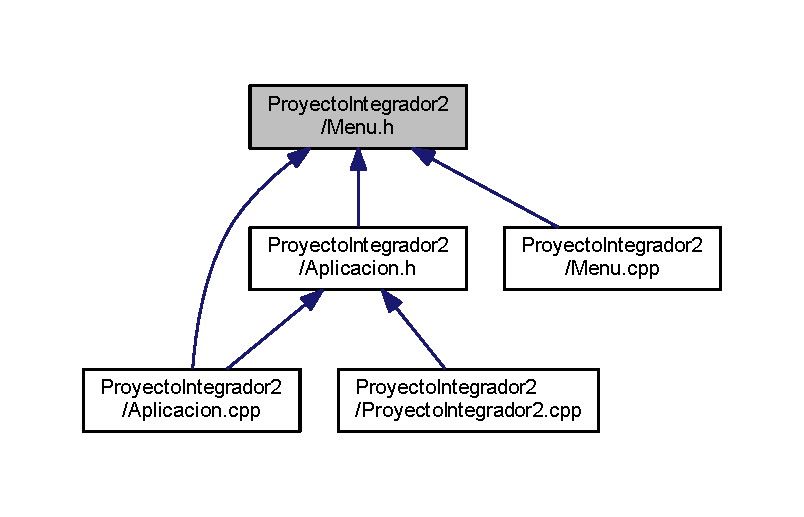
\includegraphics[width=350pt]{_menu_8h__dep__incl}
\end{center}
\end{figure}
\subsection*{Classes}
\begin{DoxyCompactItemize}
\item 
class {\bf Menu}
\end{DoxyCompactItemize}

\section{Referencia del Archivo Proyecto\-Integrador2/\-Preguntas.cpp}
\label{_preguntas_8cpp}\index{Proyecto\-Integrador2/\-Preguntas.\-cpp@{Proyecto\-Integrador2/\-Preguntas.\-cpp}}
{\ttfamily \#include \char`\"{}stdafx.\-h\char`\"{}}\\*
{\ttfamily \#include \char`\"{}Preguntas.\-h\char`\"{}}\\*
{\ttfamily \#include $<$sstream$>$}\\*
{\ttfamily \#include $<$conio.\-h$>$}\\*
{\ttfamily \#include $<$vector$>$}\\*
Dependencia gráfica adjunta para Preguntas.\-cpp\-:
\nopagebreak
\begin{figure}[H]
\begin{center}
\leavevmode
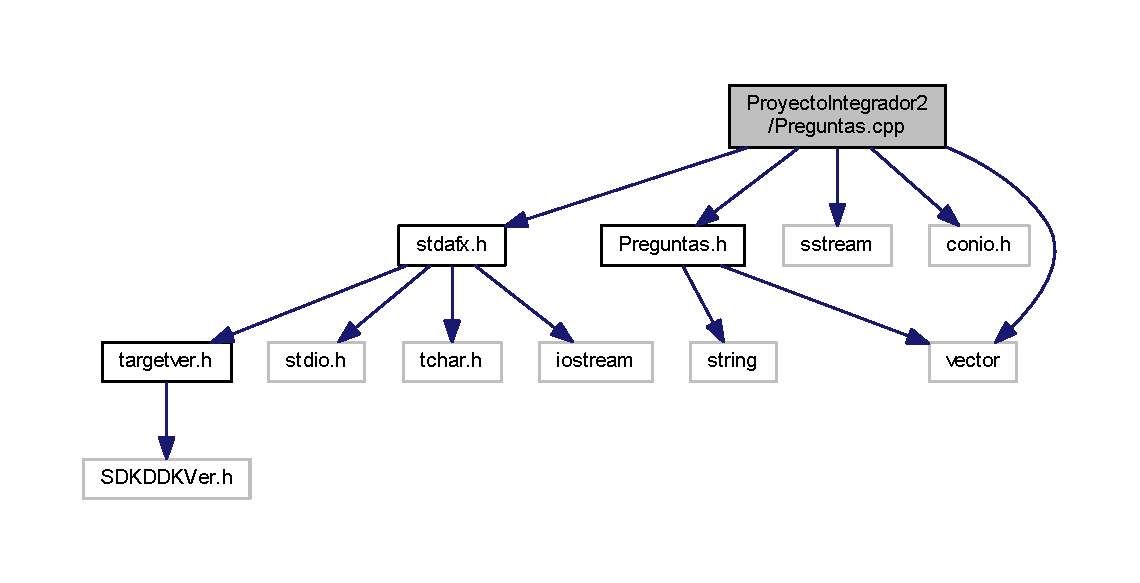
\includegraphics[width=350pt]{_preguntas_8cpp__incl}
\end{center}
\end{figure}

\section{Proyecto\-Integrador2/\-Preguntas.h File Reference}
\label{_preguntas_8h}\index{Proyecto\-Integrador2/\-Preguntas.\-h@{Proyecto\-Integrador2/\-Preguntas.\-h}}
{\ttfamily \#include $<$string$>$}\\*
{\ttfamily \#include $<$vector$>$}\\*
Include dependency graph for Preguntas.\-h\-:\nopagebreak
\begin{figure}[H]
\begin{center}
\leavevmode
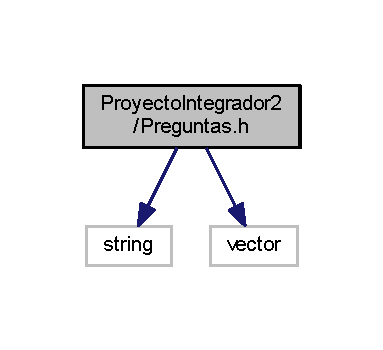
\includegraphics[width=184pt]{_preguntas_8h__incl}
\end{center}
\end{figure}
This graph shows which files directly or indirectly include this file\-:\nopagebreak
\begin{figure}[H]
\begin{center}
\leavevmode
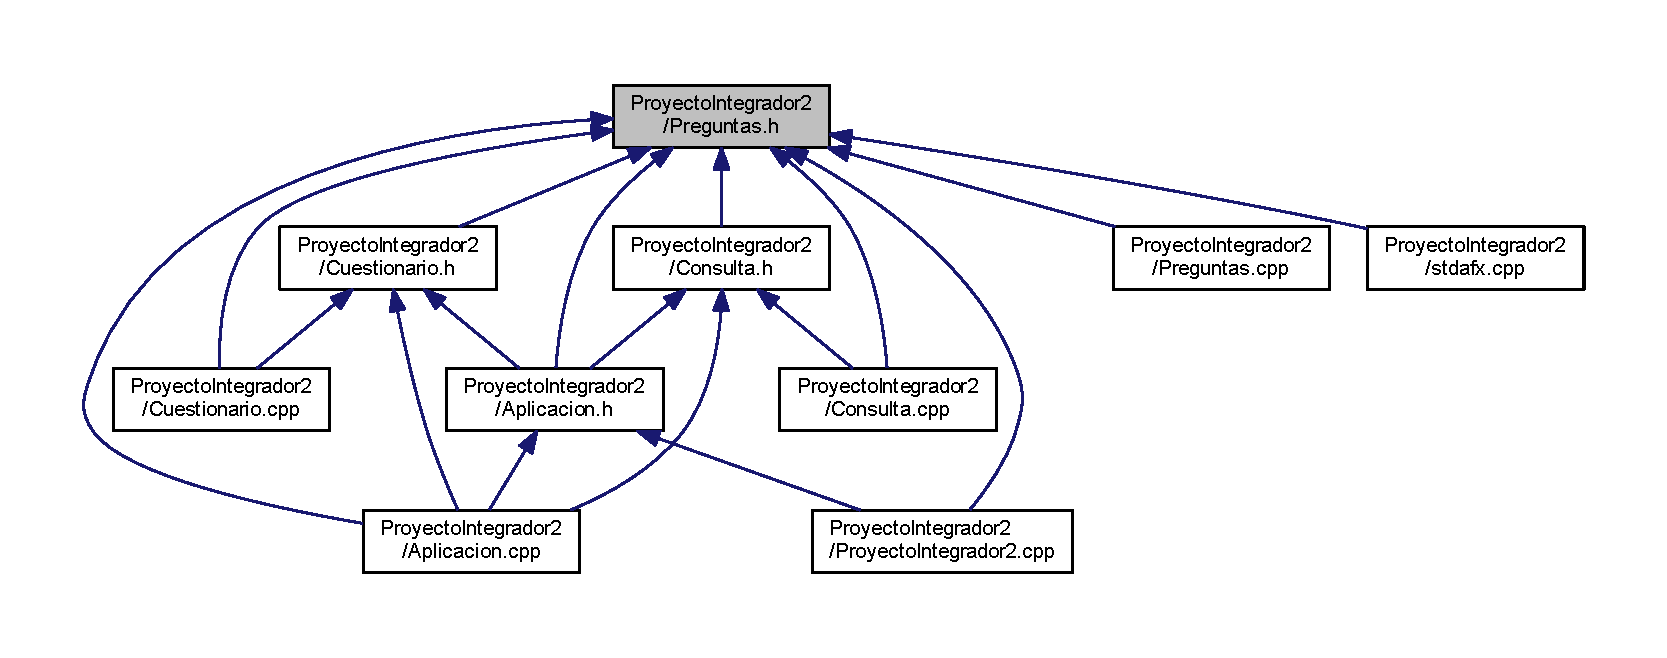
\includegraphics[width=350pt]{_preguntas_8h__dep__incl}
\end{center}
\end{figure}
\subsection*{Classes}
\begin{DoxyCompactItemize}
\item 
class {\bf Pregunta}
\item 
class {\bf Pregunta5a10}
\item 
class {\bf Pregunta\-Opc\-Mult}
\end{DoxyCompactItemize}

\section{Proyecto\-Integrador2/\-Proyecto\-Integrador2.cpp File Reference}
\label{_proyecto_integrador2_8cpp}\index{Proyecto\-Integrador2/\-Proyecto\-Integrador2.\-cpp@{Proyecto\-Integrador2/\-Proyecto\-Integrador2.\-cpp}}
{\ttfamily \#include \char`\"{}stdafx.\-h\char`\"{}}\\*
{\ttfamily \#include \char`\"{}Preguntas.\-h\char`\"{}}\\*
{\ttfamily \#include \char`\"{}Aplicacion.\-h\char`\"{}}\\*
Include dependency graph for Proyecto\-Integrador2.\-cpp\-:\nopagebreak
\begin{figure}[H]
\begin{center}
\leavevmode
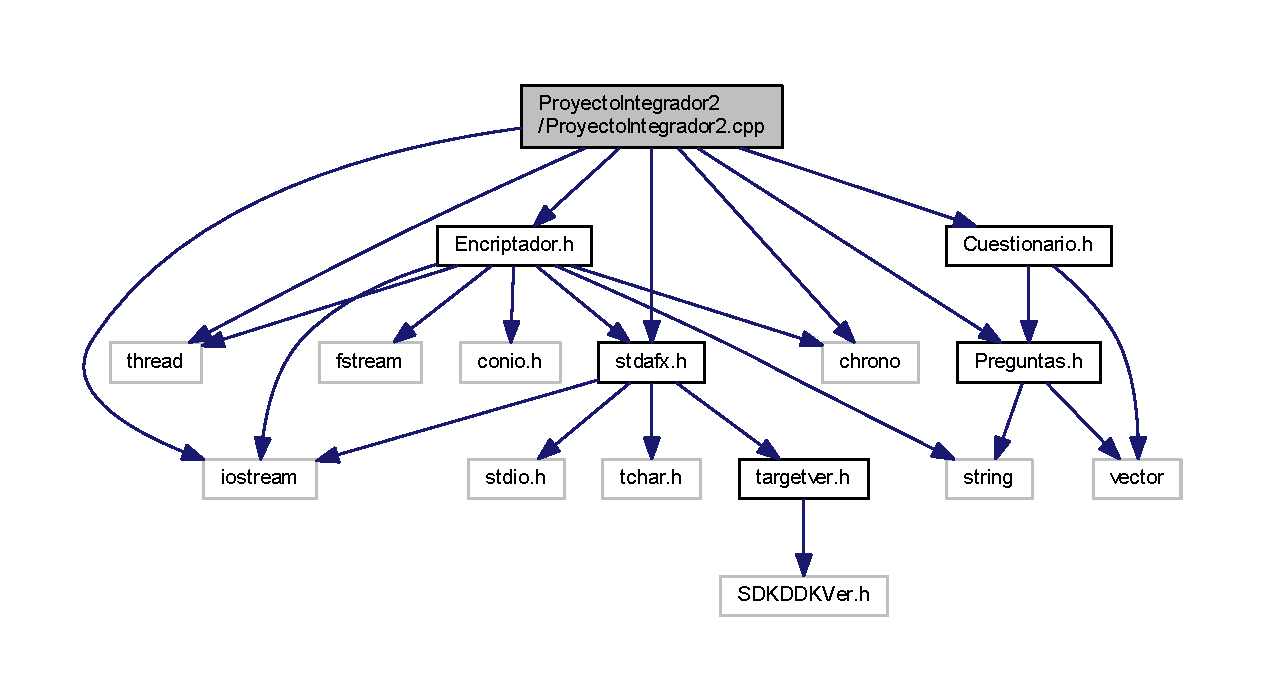
\includegraphics[width=350pt]{_proyecto_integrador2_8cpp__incl}
\end{center}
\end{figure}
\subsection*{Functions}
\begin{DoxyCompactItemize}
\item 
int {\bf \-\_\-tmain} (int argc, \-\_\-\-T\-C\-H\-A\-R $\ast$argv[$\,$])
\end{DoxyCompactItemize}


\subsection{Function Documentation}
\index{Proyecto\-Integrador2.\-cpp@{Proyecto\-Integrador2.\-cpp}!\-\_\-tmain@{\-\_\-tmain}}
\index{\-\_\-tmain@{\-\_\-tmain}!ProyectoIntegrador2.cpp@{Proyecto\-Integrador2.\-cpp}}
\subsubsection[{\-\_\-tmain}]{\setlength{\rightskip}{0pt plus 5cm}int \-\_\-tmain (
\begin{DoxyParamCaption}
\item[{int}]{argc, }
\item[{\-\_\-\-T\-C\-H\-A\-R $\ast$}]{argv[$\,$]}
\end{DoxyParamCaption}
)}\label{_proyecto_integrador2_8cpp_a353674c5af92be7fb389265cde4e5e03}


Definition at line 10 of file Proyecto\-Integrador2.\-cpp.


\begin{DoxyCode}
11 \{
12     Aplicacion programa;
13     vector<Pregunta*> preguntas; \textcolor{comment}{//Se crea un vector de punteros del tipo Pregunta, para almacenar las
       preguntas de la encuesta}
14     preguntas.push\_back(\textcolor{keyword}{new} Pregunta(\textcolor{stringliteral}{"Biblioteca"}));
15     preguntas.push\_back(\textcolor{keyword}{new} PreguntaOpcMult(\textcolor{stringliteral}{"Seleccione una Opcion"},\textcolor{stringliteral}{"Alumno Docente Investigador    Otros"})
      );
16     preguntas.push\_back(\textcolor{keyword}{new} Pregunta(\textcolor{stringliteral}{"Carrera"}));
17     preguntas.push\_back(\textcolor{keyword}{new} Pregunta(\textcolor{stringliteral}{"Semestre"}));
18     preguntas.push\_back(\textcolor{keyword}{new} Pregunta5a10(\textcolor{stringliteral}{"Instalaciones (Comodidad, Limpieza, Iluminacion, Espacios)"}));
19     preguntas.push\_back(\textcolor{keyword}{new} Pregunta(\textcolor{stringliteral}{"Que mejoras propone?"}));
20     preguntas.push\_back(\textcolor{keyword}{new} Pregunta5a10(\textcolor{stringliteral}{"Acervo Bibliografico y documental (Actualizado, Suficiente)"}));
21     preguntas.push\_back(\textcolor{keyword}{new} Pregunta(\textcolor{stringliteral}{"Que mejoras propone?"}));
22     preguntas.push\_back(\textcolor{keyword}{new} Pregunta5a10(\textcolor{stringliteral}{"Herramientas y servicios de informacion (Prestamo de
       computadoras, Consulta en el catalogo, Acceso a bases de datos)"}));
23     preguntas.push\_back(\textcolor{keyword}{new} Pregunta(\textcolor{stringliteral}{"Que mejoras propone?"}));
24     preguntas.push\_back(\textcolor{keyword}{new} Pregunta5a10(\textcolor{stringliteral}{"Servicios del Personal (Rapidez, Asesoria)"}));
25     preguntas.push\_back(\textcolor{keyword}{new} Pregunta(\textcolor{stringliteral}{"Que mejoras propone?"}));
26     \textcolor{keywordflow}{for} (\textcolor{keywordtype}{size\_t} i=0;i<preguntas.size();i++) \{programa.addPregunta(preguntas[i]);\} \textcolor{comment}{//En este ciclo se a�aden
       todas las preguntas del vector al cuestionario}
27     programa.iniciar();
28     \textcolor{keywordflow}{return} 0;
29 \}
\end{DoxyCode}


Here is the call graph for this function\-:
\nopagebreak
\begin{figure}[H]
\begin{center}
\leavevmode
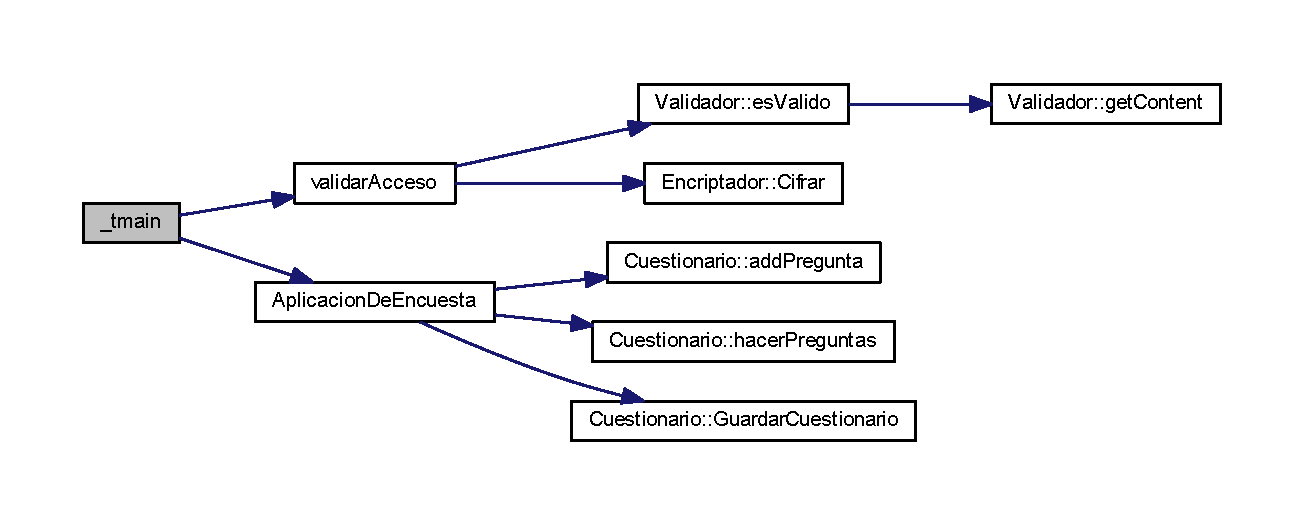
\includegraphics[width=350pt]{_proyecto_integrador2_8cpp_a353674c5af92be7fb389265cde4e5e03_cgraph}
\end{center}
\end{figure}



\section{Referencia del Archivo Proyecto\-Integrador2/stdafx.cpp}
\label{stdafx_8cpp}\index{Proyecto\-Integrador2/stdafx.\-cpp@{Proyecto\-Integrador2/stdafx.\-cpp}}
{\ttfamily \#include \char`\"{}stdafx.\-h\char`\"{}}\\*
{\ttfamily \#include \char`\"{}Preguntas.\-h\char`\"{}}\\*
{\ttfamily \#include $<$string$>$}\\*
Dependencia gráfica adjunta para stdafx.\-cpp\-:
\nopagebreak
\begin{figure}[H]
\begin{center}
\leavevmode
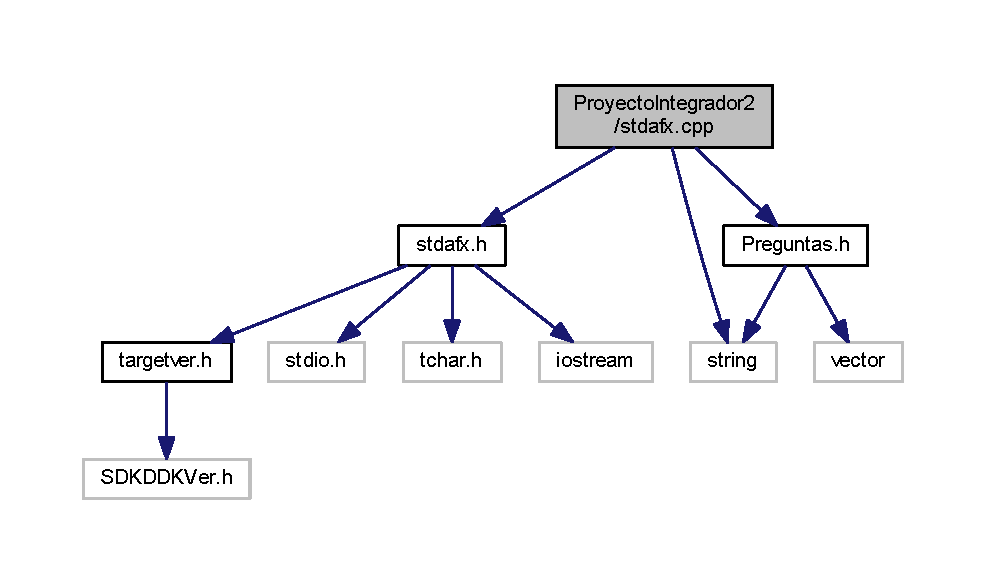
\includegraphics[width=350pt]{stdafx_8cpp__incl}
\end{center}
\end{figure}

\section{Proyecto\-Integrador2/stdafx.h File Reference}
\label{stdafx_8h}\index{Proyecto\-Integrador2/stdafx.\-h@{Proyecto\-Integrador2/stdafx.\-h}}
{\ttfamily \#include \char`\"{}targetver.\-h\char`\"{}}\\*
{\ttfamily \#include $<$stdio.\-h$>$}\\*
{\ttfamily \#include $<$tchar.\-h$>$}\\*
{\ttfamily \#include $<$iostream$>$}\\*
Include dependency graph for stdafx.\-h\-:\nopagebreak
\begin{figure}[H]
\begin{center}
\leavevmode
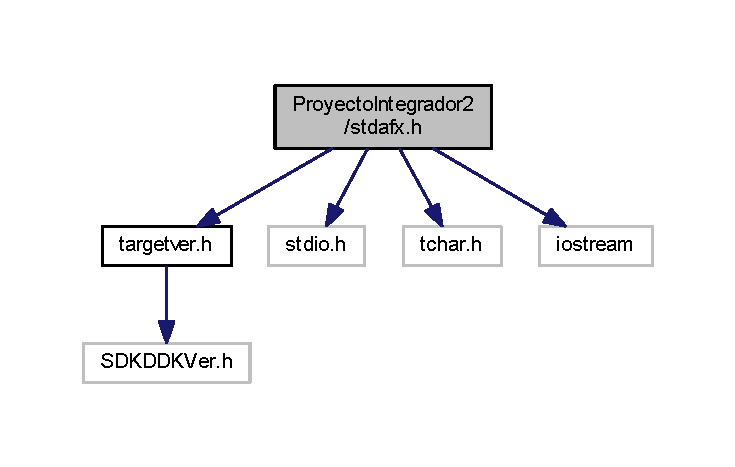
\includegraphics[width=350pt]{stdafx_8h__incl}
\end{center}
\end{figure}
This graph shows which files directly or indirectly include this file\-:\nopagebreak
\begin{figure}[H]
\begin{center}
\leavevmode
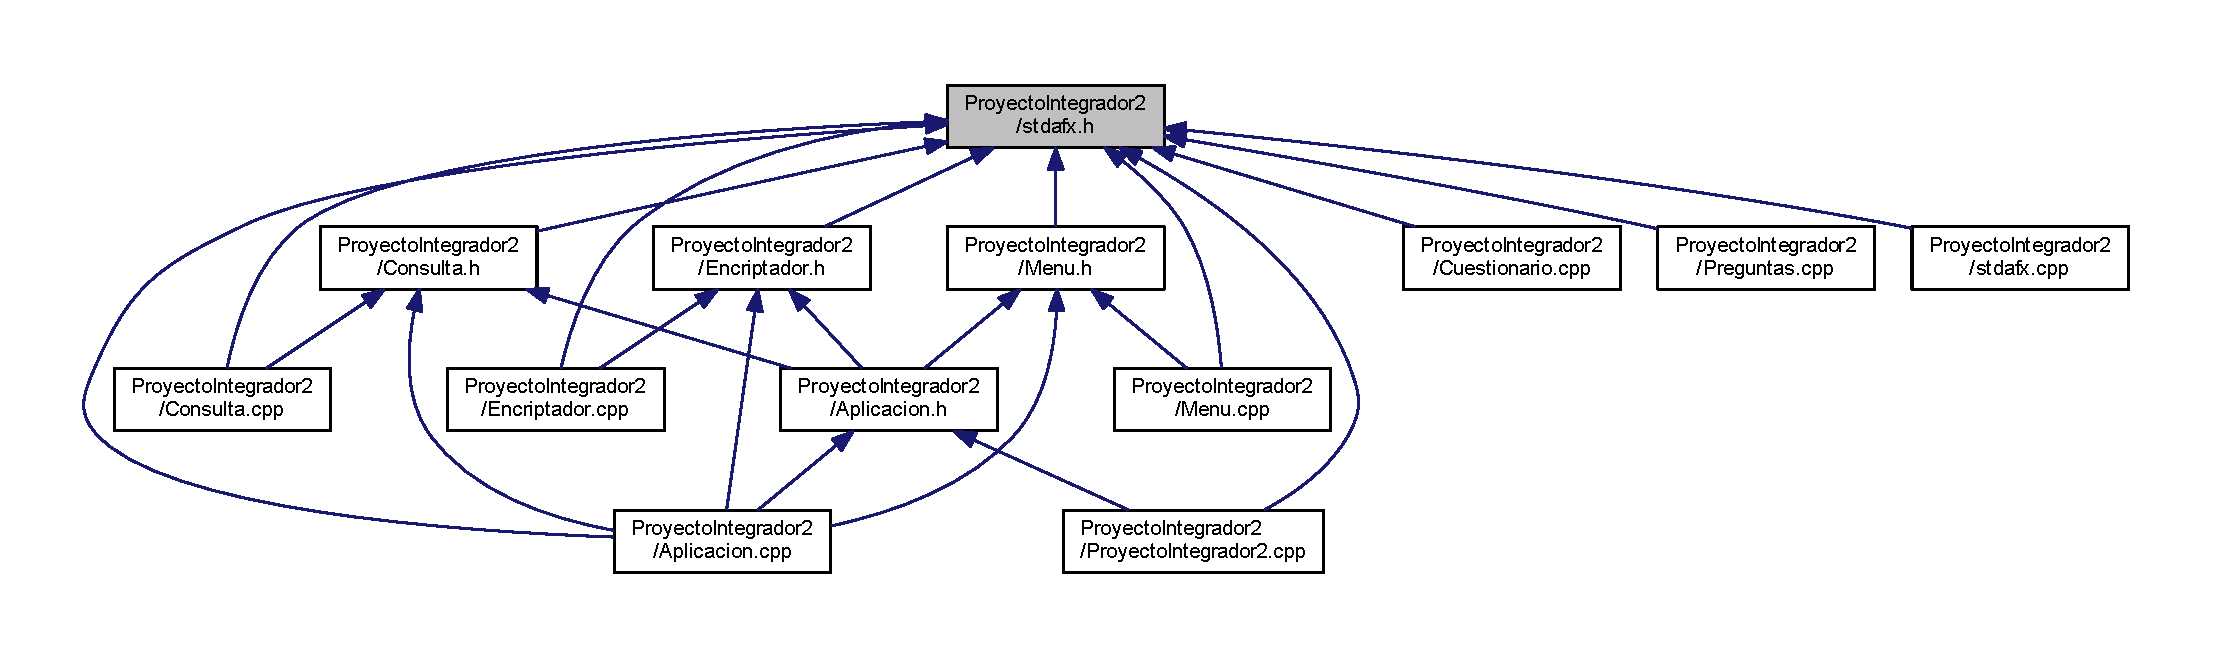
\includegraphics[width=350pt]{stdafx_8h__dep__incl}
\end{center}
\end{figure}
\subsection*{Macros}
\begin{DoxyCompactItemize}
\item 
\#define {\bf \-\_\-\-C\-R\-T\-\_\-\-S\-E\-C\-U\-R\-E\-\_\-\-N\-O\-\_\-\-W\-A\-R\-N\-I\-N\-G\-S}
\end{DoxyCompactItemize}


\subsection{Macro Definition Documentation}
\index{stdafx.\-h@{stdafx.\-h}!\-\_\-\-C\-R\-T\-\_\-\-S\-E\-C\-U\-R\-E\-\_\-\-N\-O\-\_\-\-W\-A\-R\-N\-I\-N\-G\-S@{\-\_\-\-C\-R\-T\-\_\-\-S\-E\-C\-U\-R\-E\-\_\-\-N\-O\-\_\-\-W\-A\-R\-N\-I\-N\-G\-S}}
\index{\-\_\-\-C\-R\-T\-\_\-\-S\-E\-C\-U\-R\-E\-\_\-\-N\-O\-\_\-\-W\-A\-R\-N\-I\-N\-G\-S@{\-\_\-\-C\-R\-T\-\_\-\-S\-E\-C\-U\-R\-E\-\_\-\-N\-O\-\_\-\-W\-A\-R\-N\-I\-N\-G\-S}!stdafx.h@{stdafx.\-h}}
\subsubsection[{\-\_\-\-C\-R\-T\-\_\-\-S\-E\-C\-U\-R\-E\-\_\-\-N\-O\-\_\-\-W\-A\-R\-N\-I\-N\-G\-S}]{\setlength{\rightskip}{0pt plus 5cm}\#define \-\_\-\-C\-R\-T\-\_\-\-S\-E\-C\-U\-R\-E\-\_\-\-N\-O\-\_\-\-W\-A\-R\-N\-I\-N\-G\-S}\label{stdafx_8h_af08ec37a8c99d747fb60fa15bc28678b}


Definition at line 9 of file stdafx.\-h.


\section{Referencia del Archivo Proyecto\-Integrador2/targetver.h}
\label{targetver_8h}\index{Proyecto\-Integrador2/targetver.\-h@{Proyecto\-Integrador2/targetver.\-h}}
{\ttfamily \#include $<$S\-D\-K\-D\-D\-K\-Ver.\-h$>$}\\*
Dependencia gráfica adjunta para targetver.\-h\-:
\nopagebreak
\begin{figure}[H]
\begin{center}
\leavevmode
\includegraphics[width=184pt]{targetver_8h__incl}
\end{center}
\end{figure}
Gráfico de los archivos que directa o indirectamente incluyen a este archivo\-:
\nopagebreak
\begin{figure}[H]
\begin{center}
\leavevmode
\includegraphics[width=350pt]{targetver_8h__dep__incl}
\end{center}
\end{figure}

%--- End generated contents ---

% Index
\newpage
\phantomsection
\addcontentsline{toc}{part}{Index}
\printindex

\end{document}
